\section{Kết quả đánh giá, thống kê và so sánh}

\subsection{Đánh giá mô phỏng và kết quả benchmark}

\subsubsection{Đánh giá mô phỏng và kết quả benchmark RMSE}

\hspace{0.5cm} Giai đoạn này tập trung vào việc thiết lập môi trường mô phỏng có kiểm soát hoàn toàn để đánh giá định lượng hiệu suất của hai bộ lọc alpha-beta và Kalman trên ba loại mục tiêu khác nhau. Mô phỏng cho phép lặp lại chính xác cùng một kịch bản với các thông số cố định, loại bỏ yếu tố ngẫu nhiên không kiểm soát được vốn tồn tại trong đo lường thực địa. Kết quả benchmark RMSE (Root Mean Square Error) cung cấp cơ sở so sánh khách quan giữa các phương pháp xử lý.

Phương pháp mô phỏng thuận lợi hơn thử nghiệm thực địa trong giai đoạn phát triển ban đầu. Chi phí triển khai cảm biến thực trên người đi bộ, xe máy và drone rất cao, đồng thời khó kiểm soát được các yếu tố môi trường như nhiễu GPS multipath, gió, hay điều kiện địa hình. Mô phỏng cho phép thay đổi đơn lẻ từng tham số (vận tốc mục tiêu, mức nhiễu, loại cảm biến) để đánh giá ảnh hưởng của từng yếu tố đến hiệu suất tracking, điều gần như không thể trong thực nghiệm thực địa.

Để đảm bảo tính khách quan, mỗi kịch bản mô phỏng được chạy với cùng một giá trị seed (seed = 42), tạo ra chuỗi số ngẫu nhiên cố định cho việc sinh quỹ đạo và nhiễu cảm biến. Việc sử dụng seed cố định có hai ý nghĩa: (a) kết quả có thể tái lập chính xác trên bất kỳ máy tính nào, và (b) cho phép so sánh công bằng giữa các phương pháp vì tất cả đều nhận cùng một đầu vào nhiễu. Nhược điểm của cách tiếp cận này là kết quả chỉ đại diện cho một mẫu ngẫu nhiên duy nhất; để có đánh giá tổng quát hơn, cần chạy nhiều seed khác nhau và tính trung bình cùng độ lệch chuẩn trên tập hợp kết quả.

\subsubsection{Thiết lập mô phỏng}

\hspace{0.5cm} Hệ thống mô phỏng được tổ chức theo kiến trúc ba lớp: bộ điều phối mô phỏng xử lý toàn bộ quá trình theo chu kỳ thời gian, bộ sinh quỹ đạo mục tiêu tạo quỹ đạo theo từng loại đối tượng, và bộ quản lý ranh giới áp dụng ranh giới hình tròn để giữ mục tiêu trong vùng quan sát. Kiến trúc ba lớp này tách biệt rõ ràng giữa logic mô phỏng (sinh quỹ đạo, tạo phép đo), logic xử lý (hợp nhất cảm biến, bộ lọc), và logic điều phối (quản lý phiên, thu thập thống kê).

Mỗi bước thời gian, bộ điều phối mô phỏng thực hiện theo trình tự: (1) gọi bộ sinh quỹ đạo mục tiêu để lấy vị trí mục tiêu tiếp theo trên quỹ đạo, (2) mô phỏng phép đo từ vị trí mục tiêu bằng cách thêm nhiễu cảm biến (GPS, IMU, laser) vào vị trí thực, (3) đưa phép đo mô phỏng vào khối hợp nhất cảm biến để hợp nhất thành tọa độ mục tiêu ước lượng, (4) đưa kết quả hợp nhất vào bộ lọc (alpha-beta hoặc Kalman) để lọc nhiễu và ước lượng vị trí cuối cùng, (5) ghi nhận sai số giữa vị trí thực và vị trí ước lượng để tính RMSE. Vòng lặp này chạy liên tục cho đến khi kết thúc phiên mô phỏng (1.200 bước).

Phép đo mô phỏng được tạo bằng cách mô hình hóa hoạt động của từng cảm biến. GPS mô phỏng bằng cách thêm nhiễu chuẩn $N(0, \sigma_{gps}^2)$ vào tọa độ thực. Laser mô phỏng bằng cách thêm nhiễu khoảng cách $N(0, \sigma_{laser}^2)$ vào khoảng cách thực từ người quan sát đến mục tiêu, sau đó chuyển đổi về tọa độ Cartesian. IMU mô phỏng bằng cách thêm nhiễu góc $N(0, \sigma_{az}^2)$ vào góc azimuth thực và $N(0, \sigma_{el}^2)$ vào góc elevation thực. Mỗi cảm biến được mô phỏng độc lập, không có tương tác giữa các nhiễu.

Khối hợp nhất cảm biến nhận đầu vào từ ba cảm biến (GPS, IMU, laser) và xuất ra tọa độ mục tiêu ước lượng trong hệ tọa độ ENU (East-North-Up). Quá trình hợp nhất sử dụng mô hình RSS (Revised Sum of Squares) để tính sai số tổng hợp $\sigma_{pos}$, sau đó xác định trọng số hợp nhất cho từng cảm biến. Ở khoảng cách gần (dưới 400 m), GPS chiếm trọng số lớn nhất; ở khoảng cách xa (trên 794 m), IMU chiếm ưu thế.

Kết quả mô phỏng được thu thập qua bộ đệm dạng vòng lưu trữ 500 frame gần nhất. Mỗi frame chứa: vị trí thực, vị trí đo thô, vị trí alpha-beta, vị trí Kalman, và timestamp. Bộ đệm này cung cấp dữ liệu cho các dịch vụ thống kê và xuất dữ liệu của REST và cho việc vẽ biểu đồ phân tích. Số frame 500 là đủ để bao phủ 50 giây mô phỏng tại 10 Hz, đảm bảo có đủ dữ liệu để phân tích cả hành vi ngắn hạn (đỉnh sai số) và dài hạn (xu hướng sai số).

Bộ sinh quỹ đạo mục tiêu quản lý việc tạo quỹ đạo dựa trên loại mục tiêu được chọn. Mỗi loại mục tiêu có một lớp tạo quỹ đạo riêng, được đăng ký trong ánh xạ nội bộ. Khi khởi tạo, bộ sinh quỹ đạo chọn ngẫu nhiên vị trí bắt đầu trong phạm vi ranh giới bằng hàm chọn điểm khởi đầu ngẫu nhiên trong ranh giới, tạo ra một điểm ngẫu nhiên trong đĩa bán kính $0{,}8 \cdot R_{boundary}$ (nằm trong vùng trường lực mềm). Việc khởi tạo ngẫu nhiên đảm bảo mỗi lần chạy mô phỏng (ENGAGE) tạo ra quỹ đạo khác nhau ngay cùng một loại mục tiêu và seed, tăng tính đa dạng của dữ liệu đánh giá.

Sau khi xác định vị trí bắt đầu, bộ sinh quỹ đạo tạo chuỗi điểm trên quỹ đạo với tần số mẫu 10 Hz. Mỗi điểm trên quỹ đạo được kèm theo: (a) tọa độ $(x, y)$ hoặc $(x, y, z)$, (b) vectơ vận tốc $(v_x, v_y)$ hoặc $(v_x, v_y, v_z)$, (c) góc azimuth $\theta$ để sử dụng trong mô hình cảm biến IMU. Chuỗi điểm này được lưu trong bộ đệm dạng vòng và truy xuất theo chỉ số bước thời gian.

Bộ quản lý ranh giới sử dụng mô hình trường lực mềm (soft potential field) để giữ mục tiêu trong vùng quan sát. Khi mục tiêu tiếp cận ranh giới (bán kính $r > 0{,}8 \cdot R_{boundary}$), một lực đẩy tuyến tính được áp dụng để hướng mục tiêu trở lại trung tâm. Phương pháp này tạo chuyển động tự nhiên hơn so với phản xạ cứng (hard reflection), tránh hiện tượng dao động kiểu bóng billiard khi mục tiêu chạm ranh giới.

Lực đẩy được tính theo công thức:
\begin{equation}
F_{repulse} = \begin{cases}
0 & \text{nếu } r < 0{,}8 \cdot R_{boundary} \\
k \cdot \frac{r - 0{,}8 \cdot R_{boundary}}{0{,}2 \cdot R_{boundary}} \cdot (-\hat{r}) & \text{nếu } r \geq 0{,}8 \cdot R_{boundary}
\end{cases}
\end{equation}

trong đó $k$ là hệ số lực (được đặt để tạo đẩy đủ mạnh nhưng không gây jitter), $\hat{r}$ là vectơ đơn vị hướng tâm, và $r$ là khoảng cách hiện tại đến tâm. Lực này được cộng thêm vào vectơ vận tốc của mục tiêu tại mỗi bước, tạo ra khúc rẽ mượt mà khi mục tiêu tiếp cận ranh giới.

Vùng áp dụng trường lực mềm (từ $0{,}8R$ đến $R$) chiếm 20\% bán kính ranh giới, tương đương 80 m khi $R_{boundary} = 400$ m. Trong vùng này, lực đẩy tăng tuyến tính từ 0 (tại $r = 0{,}8R$) đến giá trị lớn nhất (tại $r = R$). Sự chuyển tiếp mượt mà này đảm bảo mục tiêu không bị ảnh hưởng đột ngột khi tiếp cận ranh giới, tạo ra các khúc rẽ tự nhiên thay vì các góc nhọn bất thường. Kết quả là quỹ đạo mục tiêu luôn mượt mà ngay cả khi bị ảnh hưởng bởi trường lực đẩy.

Thông số mô phỏng chuẩn được sử dụng trong toàn bộ đánh giá được liệt kê trong Bảng \ref{tab:sim-params-week4}.

\begin{table}[H]
\centering
\caption{Thông số mô phỏng chuẩn}
\label{tab:sim-params-week4}
\adjustbox{max width=\linewidth}{
\begin{tabular}{lll}
\toprule
\textbf{Tham số} & \textbf{Giá trị} & \textbf{Ghi chú} \\
\midrule
Thời gian mô phỏng    & 120 s           & 1.200 bước tại 10 Hz \\
Tần số mẫu            & 10 Hz           & 0,1 s mỗi bước \\
Bán kính ranh giới    & 400 m           & Giới hạn vùng quan sát \\
Giá trị khởi tạo (seed) & 42           & Đảm bảo tính tái lập \\
Tọa độ người quan sát & (10,7626$^\circ$N, 106,6602$^\circ$E) & Quận 10, TP.HCM \\
\bottomrule
\end{tabular}
}
\end{table}

Bốn tham số chuẩn ở trên không được chọn tùy tiện. Giá trị khởi tạo $42$ cố định biến ngẫu nhiên của tất cả phép đo, nhờ đó mọi lần chạy với cùng cấu hình đều sinh ra đúng một chuỗi nhiễu như nhau. Số cụ thể $42$ tự nó không mang ý nghĩa vật lý; nó chỉ phục vụ việc khóa nguồn nhiễu để so sánh công bằng giữa các phương pháp lọc trên cùng một tín hiệu đầu vào.

Thời gian $120$ giây tương ứng $1.200$ bước ở tần số cập nhật $10$ Hz. Độ dài này đủ để bộ lọc Kalman rời khỏi giai đoạn hội tụ ban đầu (quan sát được trong khoảng $15$ đến $20$ giây đầu) và đạt trạng thái ổn định, đồng thời vẫn ngắn gọn để trình diễn tương tác theo thời gian thực mà không rời rạc. Người đi bộ, xe máy và drone đều có dịp băng qua đầy đủ các quy luật chuyển động riêng của mình trong khoảng thời gian này.

Tần số $10$ Hz là nhịp đầu ra của khối hợp nhất cảm biến chứ không phải lời khẳng định về bản thân cảm biến. Sau khi nội suy, các tập dữ liệu thực (đi bộ của Geolife lấy mẫu thô $1$ đến $5$ giây, xe máy của AMIT lấy mẫu $5$ Hz) được đưa về lưới thời gian chung $10$ Hz trước khi cập nhật bộ lọc. Giá trị $10$ Hz nằm ở vùng dung hòa giữa độ mịn của quỹ đạo và khối lượng tính toán trong mỗi chu kỳ $100$ ms.

Bán kính ranh giới $400$ m thể hiện tầm hoạt động hiệu dụng của thiết bị đo khoảng cách laser, nằm trong dải thiết kế $[100, 1000]$ m đã nêu và bao trùm biên chuyển động của cả ba loại mục tiêu. Ở phạm vi này, trường lực mềm bắt đầu tác động từ $0{,}8 \times 400 = 320$ m, cho phép quan sát rõ hành vi khi mục tiêu tiến gần rìa vùng.

Mô hình nhiễu cảm biến được mô tả trong Bảng \ref{tab:noise-week4}. Mỗi cảm biến có mô hình nhiễu riêng: GPS có nhiễu chuẩn $\sigma_{GPS}$ trên cả hai trục ngang, IMU có nhiễu góc azimuth và elevation, laser có nhiễu khoảng cách. Các nhiễu này được thêm vào phép đo mô phỏng để mô phỏng điều kiện đo lường thực tế.

\begin{table}[H]
\centering
\caption{Thông số nhiễu cảm biến trong mô phỏng}
\label{tab:noise-week4}
\adjustbox{max width=\linewidth}{
\begin{tabular}{lcc}
\toprule
\textbf{Cảm biến} & \textbf{Thông số} & \textbf{Giá trị} \\
\midrule
GPS/GNSS       & $\sigma_{GPS}$     & 5,0 m          \\
IMU (azimuth)  & $\sigma_{az}$      & 0,3$^\circ$    \\
IMU (elevation)& $\sigma_{el}$      & 0,2$^\circ$    \\
Laser          & $\sigma_{laser}$   & 0,5 m          \\
\bottomrule
\end{tabular}
}
\end{table}

Ba loại mục tiêu được mô phỏng tương ứng với ba trường hợp sử dụng thực tế: người đi bộ (Kalman 2D), xe máy (Kalman 2D), và drone (Kalman 3D với trục Up). Mỗi loại mục tiêu có mô hình chuyển động và mức độ cơ động khác nhau, phản ánh các điều kiện tracking đa dạng trong thực tế.

Mối quan hệ giữa loại mục tiêu và loại Kalman filter là do đặc tính chuyển động: người đi bộ và xe máy di chuyển trên mặt phẳng ngang (2D), nên Kalman filter chỉ cần trạng thái $(x, y, v_x, v_y)$. Drone bay trong không gian 3D với thay đổi độ cao liên tục, nên cần thêm trạng thái $(z, v_z)$ để mô tả thành phần thẳng đứng. Sự khác biệt về chiều không gian ảnh hưởng đến kích thước ma trận trạng thái ($4 \times 4$ cho 2D, $6 \times 6$ cho 3D), ma trận đo lường, và ma trận nhiễu quá trình, tạo ra sự phức tạp hơn đáng kể cho Kalman 3D.

\subsubsection{Mô hình mục tiêu người đi bộ}

\hspace{0.5cm} Mô hình người đi bộ mô phỏng chuyển động của một người đi bộ với các đặc điểm vi mô vật lý. Mô hình tạo quỹ đạo tuyến tính cơ bản và bổ sung các yếu tố động học thực tế như nhiễu góc heading theo quá trình Ornstein-Uhlenbeck (OU), điều chỉnh nhịp bước (gait modulation), và các sự kiện dừng lại (pause events). Tổng hợp ba yếu tố này tạo ra quỹ đạo có độ tin cậy cao, phản ánh đúng hành vi đi bộ trong đô thị.

Quỹ đạo được tạo theo từng bước thời gian, với vận tốc tuyến tính hướng về mục tiêu tiếp theo được điều chỉnh bởi góc heading OU. Tại mỗi bước, góc heading mới được tính bằng cách cộng thêm nhiễu OU vào góc trước đó:
\begin{equation}
\theta_k = \theta_{k-1} + \frac{1}{\tau}\left(\mu_\theta - \theta_{k-1}\right)\Delta t + \sigma_\theta \sqrt{\Delta t}\, W_k,
\end{equation}

trong đó $\mu_\theta$ là góc heading trung bình (hướng về mục tiêu), $\tau$ là thời gian tự tương quan, $\sigma_\theta$ là biên độ nhiễu, và $W_k$ là biến chuẩn hóa $N(0,1)$. Hệ số $\frac{1}{\tau}$ đảm bảo góc heading có xu hướng quay về hướng mục tiêu, trong khi số hạng $\sigma_\theta \sqrt{\Delta t}\, W_k$ thêm nhiễu ngẫu nhiên.

Hiệu ứng OU tạo ra các đoạn đi thẳng dài xen kẽ với các khúc rẽ mượt mà. Khi $\tau$ lớn, góc heading thay đổi chậm và quỹ đạo có các đoạn thẳng dài (phù hợp với đi bộ trên đường thẳng). Khi $\tau$ nhỏ, góc heading thay đổi nhanh và quỹ đạo có nhiều khúc rẽ (phù hợp với đi bộ trong khu vực đông đúc). Với $\tau = 1{,}0$ s, mô hình tạo ra quỹ đạo có độ dài đoạn thẳng trung bình khoảng 1,4 m (tương đương 1 giây đi bộ), phù hợp với hành vi đi bộ trong đô thị.

Để tạo mục tiêu tiếp theo trên quỹ đạo, mô hình sử dụng chiến lược waypoints tương đối (relative waypoints). Thay vì đặt mục tiêu tại một tọa độ cố định trên bản đồ (gây ra hành vi quay đầu bất tự nhiên khi mục tiêu đến gần), mô hình chọn mục tiêu tiếp theo bằng cách cộng thêm một vectơ ngẫu nhiên vào vị trí hiện tại. Vectơ này có độ dài từ 5-15 m và hướng ngẫu nhiên, tạo ra quỹ đạo đi bộ tự nhiên với các khúc rẽ đa dạng. Khi mục tiêu tiến gần ranh giới vùng mô phỏng, hướng di chuyển được điều chỉnh dần theo lực đẩy của trường thế năng thay vì quay đầu đột ngột.

Nhiễu góc heading theo quá trình OU mô phỏng sự thay đổi hướng đi tự nhiên của người đi bộ. Thay vì sử dụng nhiễu trắng (mỗi bước chọn hướng ngẫu nhiên hoàn toàn), quá trình OU tạo chuỗi góc heading có tính tự tương quan: hướng đi tại bước thời gian $t$ có liên hệ với hướng tại bước $t-1$, với thời gian tự tương quan $\tau = 1{,}0$ s. Điều này tạo ra các đoạn đi thẳng dài xen kẽ với các khúc rẽ mượt mà, tương tự cách người đi bộ thực sự thay đổi hướng.

Điều chỉnh nhịp bước mô phỏng sự thay đổi vận tốc trong chu kỳ đi bộ. Người đi bộ không di chuyển với vận tốc hoàn toàn không đổi mà có dao động nhỏ trong mỗi chu kỳ bước chân: vận tốc tăng nhẹ khi chân bước tới và giảm khi chân nâng lên. Mô hình áp dụng dao động sin với biên độ nhỏ lên vận tốc tuyến tính, tạo quỹ đạo có nhịp điệu tự nhiên. Công thức điều chỉnh:
\begin{equation}
v_{gait}(t) = v_{mean} + A_{gait} \sin\left(\frac{2\pi t}{T_{gait}}\right),
\end{equation}
trong đó $v_{mean}$ là vận tốc trung bình, $A_{gait} = 0{,}1$ m/s là biên độ dao động, và $T_{gait} \approx 0{,}5$ s là chu kỳ đi bộ (tần số khoảng 2 Hz, tương ứng 2 bước/giây). Dao động này quá nhỏ để ảnh hưởng đáng kể đến RMSE tổng thể, nhưng tạo ra quỹ đạo có độ tin cậy cao hơn khi so sánh với quỹ đạo tuyến tính đơn giản.

Các sự kiện dừng lại mô phỏng việc người đi bộ tạm dừng trong quá trình di chuyển. Với xác suất nhỏ tại mỗi bước thời gian ($p = 0{,}02$, tương ứng khoảng 24 lần dừng trong 1.200 bước), mô hình có thể kích hoạt một khoảng dừng kéo dài từ 1 đến 5 giây (ngẫu nhiên). Trong khoảng dừng, vận tốc giảm về không theo hàm cosine trong 0,5 giây đầu, sau đó giữ nguyên ở 0, và tăng lại theo hàm cosine trong 0,5 giây cuối khi di chuyển tiếp tục. Vị trí không thay đổi trong suốt khoảng dừng.

Các sự kiện này tạo ra các đoạn quỹ đạo phẳng trên biểu đồ vị trí, phản ánh hành vi dừng lại chờ đèn đỏ hoặc nhìn đường. Từ quan điểm đánh giá bộ lọc, các khoảng dừng là thách thức: khi mục tiêu dừng lại, vận tốc thực bằng 0 nhưng bộ lọc CV vẫn dự báo vận tốc khác 0, tạo sai lệch. Alpha-beta xử lý tốt hơn ở đây vì $\beta$ nhỏ tự động giảm vận tốc ước lượng khi sai lệch đo lường nhỏ và liên tục. Kalman filter cũng xử lý được nhưng cần nhiều bước hơn để vận tốc ước lượng hội tụ về 0.

Thông số mô hình người đi bộ được tóm tắt trong Bảng \ref{tab:ped-params}.

\begin{table}[H]
\centering
\caption{Thông số mô hình người đi bộ}
\label{tab:ped-params}
\adjustbox{max width=\linewidth}{
\begin{tabular}{lll}
\toprule
\textbf{Tham số} & \textbf{Giá trị} & \textbf{Ghi chú} \\
\midrule
Vận tốc trung bình ($v_{mean}$) & 1,4 m/s & Tốc độ đi bộ bình thường \\
Tốc độ tối đa ($v_{max}$)       & 2,0 m/s & Giới hạn trên \\
Thời gian tự tương quan OU ($\tau$) & 1,0 s & Nhiễu góc heading \\
Biên độ dao động gait            & 0,1 m/s & Amplitude gait modulation \\
Xác suất dừng mỗi bước          & 0,02    & Khoảng dừng 1-5 s \\
\bottomrule
\end{tabular}
}
\end{table}

\subsubsection{Mô hình mục tiêu xe máy}

\hspace{0.5cm} Mô hình xe máy sử dụng hai cơ chế tạo quỹ đạo tùy thuộc vào chế độ dữ liệu. Trong chế độ dữ liệu thực (Real-World Data), bộ tải mạng lưới đường bộ tải mạng lưới đường thực từ tệp dữ liệu đồ thị mạng lưới đường (mạng lưới đường Thành phố Hồ Chí Minh từ OpenStreetMap) và tạo quỹ đạo bằng cách đi ngẫu nhiên (random walk) trên các đường thực. Ở chế độ tổng hợp (Synthetic), mô hình động học xe hai bánh (kinematic bicycle) được dùng để tạo quỹ đạo mượt mà với các giới hạn vận tốc và gia tốc.

Trong chế độ mạng lưới đường thực, bộ tải mạng lưới đường bộ chọn ngẫu nhiên một nút khởi đầu trong mạng lưới đường, sau đó thực hiện chuỗi bước đi ngẫu nhiên (random walk) trên các cạnh đường. Tại mỗi giao lộ, xe máy chọn một hướng đi ngẫu nhiên trong số các hướng có thể đi được. Quá trình backtracking được triển khai để tránh xe máy bị kẹt tại các nút cuối đường (dead-end): khi không có hướng đi mới, xe máy quay lại theo toàn bộ lộ trình đã đi trước đó. Độ dài trung bình của quỹ đạo khoảng 256 nút, tương đương quãng đường 2-3 km.

Độ dài quỹ đạo bị ảnh hưởng bởi mật độ mạng lưới đường. Ở khu vực trung tâm thành phố, mật độ giao lộ cao nên quỹ đạo có nhiều khúc rẽ, trong khi khu vực ngoại ô có các đoạn đường thẳng dài hơn. Việc backtracking qua toàn bộ lộ trình (thay vì chỉ 5 nút cuối cùng như phiên bản trước) đã cải thiện đáng kể: tỷ lệ quỹ đạo quá ngắn (dưới 50 nút) giảm từ 30\% xuống còn 15\%, và độ dài trung bình tăng từ 180 lên 256 nút.

Mỗi giao lộ trong mạng lưới đường có dữ liệu về loại đường (primary, secondary, tertiary), được sử dụng để điều chỉnh vận tốc. Đường chính (primary) cho phép vận tốc cao (10-12 m/s), đường secondary cho phép vận tốc trung bình (7-9 m/s), và đường tertiary cho phép vận tốc thấp (5-7 m/s). Việc điều khiển vận tốc theo loại đường tạo ra quỹ đạo có tính thực tế cao, phản ánh cách xe máy thực sự di chuyển trong đô thị: nhanh trên đường lớn, chậm trên đường nhỏ.

Vận tốc xe máy được kiểm soát theo loại đường. Trên đường chính, vận tốc trung bình khoảng 10-12 m/s (36-43 km/h); trên đường phụ, khoảng 5-8 m/s (18-29 km/h). Sự thay đổi vận tốc diễn ra mượt mà theo hàm exponential relaxation với hằng số thời gian $\tau = 2{,}0$ s, tránh các nhảy vận tốc đột ngột không vật lý. Công thức relaxation:
\begin{equation}
v_k = v_{k-1} + \frac{1}{\tau}\left(v_{target} - v_{k-1}\right)\Delta t,
\end{equation}

trong đó $v_{target}$ là vận tốc mục tiêu theo loại đường, $\tau = 2{,}0$ s là hằng số thời gian relaxation. Khi $\tau$ nhỏ, xe máy thay đổi vận tốc nhanh nhưng có thể gây giật; khi $\tau$ lớn, thay đổi mượt mà nhưng phản ứng chậm với thay đổi loại đường.

Hàm exponential relaxation tạo ra đường cong vận tốc có dạng "S-curve": vận tốc bắt đầu thay đổi chậm, sau đó nhanh, và cuối cùng chậm lại khi tiếp cận giá trị mục tiêu. Dạng này tương tự cách tài xế thực tăng tốc hoặc phanh: từ từ nhấn ga, đạt gia tốc cực đại, rồi giảm ga khi đến tốc độ mong muốn. Với $\tau = 2{,}0$ s, xe máy cần khoảng 4-6 giây (2-3$\tau$) để chuyển từ vận tốc này sang vận tốc khác, phù hợp với hành vi lái xe thực tế trong đô thị.

Mô hình kinematic bicycle ở chế độ tổng hợp sử dụng phương trình trạng thái:
\begin{equation}
\begin{aligned}
x_{k+1} &= x_k + v_k \cos(\theta_k) \cdot \Delta t \\
y_{k+1} &= y_k + v_k \sin(\theta_k) \cdot \Delta t \\
\theta_{k+1} &= \theta_k + \frac{v_k}{L} \tan(\delta_k) \cdot \Delta t
\end{aligned}
\end{equation}

trong đó $v_k$ là vận tốc, $\theta_k$ là góc heading, $\delta_k$ là góc lái, và $L = 1{,}4$ m là chiều dài cơ sở (wheelbase). Góc lái $\delta_k$ được tạo ngẫu nhiên với biên độ nhỏ ($\pm 5^\circ$), tạo ra các khúc rẽ nhẹ mô phỏng hành vi điều khiển xe trên đường thẳng.

Mô hình này tạo ra quỹ đạo có các khúc rẽ đặc trưng của xe hai bánh, khác với chuyển động tuyến tính của người đi bộ. Hiệu ứng caster trail tự nhiên: xe máy có xu hướng giữ hướng đi hiện tại khi vận tốc cao và rẽ dễ hơn khi vận tốc thấp. Điều này phản ánh đúng vật lý xe hai bánh trong thực tế, nơi centripetal force cần được cân bằng bởi moment của trọng lực để giữ thăng bằng.

\subsubsection{Mô hình mục tiêu drone}

\hspace{0.5cm} Mô hình chuyển động của drone (dựa trên mô hình động học) được thiết kế dựa trên tham số kinematic thực của khung máy bay DJI Matrice 100. Mô hình này áp dụng các giới hạn vận tốc và gia tốc từ đặc tính bay thực của drone, tạo quỹ đạo có cơ sở vật lý thay vì quỹ đạo tuyến tính đơn giản. Việc sử dụng tham số thực từ Rodrigues et al. (2021) đảm bảo quỹ đạo mô phỏng phản ánh đúng khả năng bay của drone thực tế.

Vận tốc ngang tối đa ($V_{MAX\_H}$) được đặt là 15 m/s (54 km/h), tương ứng với tốc độ bay cruise của DJI Matrice 100. Vận tốc lên cực đại ($V_{MAX\_ASC}$) là 5 m/s, phản ánh khả năng tăng độ cao của khung máy bay thực. Gia tốc ngang tối hạn là 3,0 m/s$^2$, và gia tốc thẳng đứng là 2,0 m/s$^2$. Các giới hạn này được áp dụng tại mỗi bước thời gian để đảm bảo quỹ đạo luôn khả thi về mặt vật lý. Nếu vận tốc hiện tại cộng thêm gia tốc vượt quá giới hạn, gia tốc bị cắt để giữ vận tốc trong phạm vi cho phép.

Các giới hạn kinematic này có ý nghĩa vật lý quan trọng. $V_{MAX\_H} = 15$ m/s tương đương khoảng 54 km/h, là vận tốc cruise của DJI Matrice 100 trong điều kiện bay thông thường. $V_{MAX\_ASC} = 5$ m/s phản ánh giới hạn motor: drone không thể tăng độ cao quá nhanh vì sẽ mất độ ổn định và tiêu hao năng lượng lớn. Gia tốc ngang 3,0 m/s$^2$ tương đương khả năng thay đổi hướng nhanh (sharp turns) ở vận tốc cruise, phù hợp với các tình huống theo dõi mục tiêu cơ động.

Mô hình 3D bao gồm ba thành phần vị trí: trục East (m), trục North (m), và trục Up (độ cao). Quỹ đạo được tạo bằng cách sử dụng quá trình OU cho vận tốc ngang, kết hợp với điều khiển độ cao mô phỏng. Độ cao drone dao động trong khoảng 20-100 m, với tốc độ thay đổi bị giới hạn bởi $V_{MAX\_ASC}$. Nhiễu vận tốc OU ($\tau = 1{,}0$ s) thay thế cho nhiễu bước cũ $N(0, 0{,}3)$ m/s, tạo ra các dao động vận tốc mượt mà thay vì các nhảy ngẫu nhiên tại mỗi bước. Sự thay đổi này giảm jitter đáng kể trên quỹ đạo và đưa mô hình drone đến gần hơn với hành vi bay thực.

Mô hình drone có hai cơ chế điều khiển độ cao: chế độ duy trì độ cao (altitude hold) và chế độ bay tự do. Ở chế độ duy trì độ cao, drone cố gắng giữ độ cao mục tiêu với độ dao động nhỏ. Ở chế độ bay tự do, độ cao thay đổi theo mô hình OU, tạo quỹ đạo 3D phong phú với các đoạn lên xuống tự nhiên. Trong mô phỏng benchmark, chế độ bay tự do được sử dụng để tạo quỹ đạo có tính cơ động cao hơn, thách thức khả năng theo dõi của bộ lọc.

Độ cao drone là yếu tố quan trọng ảnh hưởng đến hiệu suất tracking. Khi drone bay cao, khoảng cách slant-range từ người quan sát đến drone tăng, làm tăng thành phần IMU trong sai số hợp nhất cảm biến. Đồng thời, drone bay cao thường có vận tốc ngang lớn hơn, tạo sai lệch mô hình CV lớn hơn. Hai yếu tố này kết hợp giải thích tại sao drone có RMSE cao nhất trong ba kịch bản mục tiêu.

Thông số mô hình drone được tóm tắt trong Bảng \ref{tab:drone-kinematic-limits}.

\subsubsection{Kết quả RMSE benchmark}

\hspace{0.5cm} Bảng \ref{tab:rmse-week4} tổng hợp RMSE ngang (horizontal) của ba phương pháp xử lý trên ba kịch bản mục tiêu. Chỉ tiêu yêu cầu của đề tài là RMSE $<$ 5 m trong phạm vi 500 m. Giá trị RMSE được tính từ sai số Euclidean trung bình phương trên toàn bộ 1.200 bước thời gian, với giá trị khởi tạo seed = 42.

\begin{table}[H]
\centering
\caption{RMSE ngang của ba bộ lọc trên ba kịch bản mục tiêu (seed = 42)}
\label{tab:rmse-week4}
\adjustbox{max width=\linewidth}{
\begin{tabular}{lcccc}
\toprule
\textbf{Kịch bản} & \textbf{Đo thô} & \textbf{Alpha-beta} & \textbf{Kalman} & \textbf{Yêu cầu} \\
\midrule
Người đi bộ & 0,48 m & \textbf{0,26 m} & 0,86 m & $<$ 5 m \checkmark \\
Xe máy      & 1,89 m & \textbf{1,02 m} & 1,80 m & $<$ 5 m \checkmark \\
Drone       & 1,94 m & \textbf{1,06 m} & 2,10 m & $<$ 5 m \checkmark \\
\bottomrule
\end{tabular}
}
\end{table}

Thuật ngữ "đo thô" (raw measurements) ở đây chỉ vị trí tính trực tiếp từ hợp nhất cảm biến (kết hợp GPS, IMU, laser) có nhiễu, chưa qua bất kỳ bộ lọc nào. Đo thô đại diện cho chất lượng đầu vào trước khi xử lý, trong khi các giá trị alpha-beta và Kalman là kết quả sau khi lọc. Sự khác biệt giữa "đo thô" và "đã lọc" chính là giá trị mà bộ lọc mang lại: giảm nhiễu, mượt hóa quỹ đạo, và ước lượng vận tốc.

Từ kết quả RMSE, có thể tính tỷ lệ cải thiện (improvement ratio) của mỗi bộ lọc so với đo thô:
\begin{equation}
IR = \frac{RMSE_{raw} - RMSE_{filtered}}{RMSE_{raw}} \times 100\%.
\end{equation}

Áp dụng cho từng trường hợp: alpha-beta cải thiện 46\% (người đi bộ), 46\% (xe máy), 45\% (drone); Kalman cải thiện 41\% (người đi bộ), nhưng kém hơn đo thô ở xe máy và drone. Tỷ lệ cải thiện gần như không đổi ở alpha-beta cho thấy bộ lọc hoạt động ổn định bất kể loại mục tiêu, trong khi tỷ lệ cải thiện của Kalman phụ thuộc mạnh vào sự phù hợp giữa mô hình DWNA và đặc tính chuyển động thực.

Cả ba kịch bản đều đạt yêu cầu bài toán (RMSE $<$ 5 m). Alpha-beta filter đạt RMSE thấp nhất ở cả ba trường hợp, với cải thiện từ 46\% đến 47\% so với đo thô. Kalman filter cải thiện hơn so với đo thô ở người đi bộ (cải thiện 41\% so với đo thô), nhưng hiệu suất kém hơn ở xe máy và drone. Hình \ref{fig:rmse-bar} biểu diễn so sánh trực quan RMSE giữa ba phương pháp.

Tỷ lệ cải thiện giữa alpha-beta và Kalman quan trọng nhất ở drone (alpha-beta thấp hơn 50\% so với Kalman), trong khi ở người đi bộ, khoảng cách nhỏ hơn (alpha-beta thấp hơn 70\% so với Kalman). Điều này cho thấy sự khác biệt giữa hai bộ lọc tăng lên khi tính cơ động của mục tiêu tăng: drone có chuyển động 3D với thay đổi độ cao liên tục, tạo ra sai lệch mô hình lớn hơn so với mô hình CV mà cả hai bộ lọc đều giả định.

\subsubsection{Biểu đồ RMSE benchmark}

\hspace{0.5cm} Hình \ref{fig:rmse-bar} vẽ biểu đồ cột so sánh RMSE ngang giữa ba phương pháp trên ba kịch bản mục tiêu. Biểu đồ sử dụng ba màu phân biệt: xám cho đo thô, xanh dương cho alpha-beta, và đỏ cho Kalman. Giá trị RMSE được hiển thị trên từng cột để dễ so sánh trực tiếp.

\begin{figure}[H]
\centering
\includegraphics[width=0.92\textwidth]{figures/rmse_comparison_bar.png}
\caption{So sánh RMSE ngang giữa ba phương pháp trên ba kịch bản mục tiêu}
\label{fig:rmse-bar}
\end{figure}

Nhìn vào biểu đồ, có thể thấy rõ mô hình: alpha-beta luôn đạt RMSE thấp nhất, đo thô ở mức trung bình, và Kalman có RMSE cao nhất ở hai kịch bản xe máy và drone. Chỉ ở kịch bản người đi bộ, Kalman có RMSE cao hơn đáng kể so với đo thô, cho thấy bộ lọc Kalman chưa tối ưu cho mục tiêu có vận tốc thấp.

Một quan sát là khoảng cách RMSE giữa alpha-beta và Kalman tăng dần từ người đi bộ đến drone. Ở người đi bộ, khoảng cách là $0{,}86 - 0{,}26 = 0{,}60$ m; ở xe máy, $1{,}80 - 1{,}02 = 0{,}78$ m; ở drone, $2{,}10 - 1{,}06 = 1{,}04$ m. Xu hướng này cho thấy sự khác biệt giữa hai bộ lọc trở nên rõ ràng hơn khi tính cơ động của mục tiêu tăng. Drone có chuyển động 3D với thay đổi độ cao liên tục, tạo ra sai lệch mô hình CV lớn nhất, và Kalman filter với mô hình DWNA fixed-rate xử lý kém hơn alpha-beta filter vốn tự điều chỉnh qua sai lệch đo lường.

Một quan sát khác là cải thiện của alpha-beta so với đo thô gần như không đổi qua ba kịch bản (46\%, 46\%, 45\%). Điều này cho thấy alpha-beta filter hoạt động độc lập với đặc tính chuyển động của mục tiêu: dù mục tiêu đi bộ (1,4 m/s), chạy xe máy (5-12 m/s), hay bay drone (15 m/s), bộ lọc luôn cải thiện khoảng 46\% so với đo thô. Tính ổn định này là lợi thế lớn khi triển khai thực tế, nơi đặc tính chuyển động của mục tiêu thường không biết trước.

\subsubsection{Phân tích đường cong sai số theo thời gian}

\hspace{0.5cm} Biểu đồ đường cong sai số theo thời gian (error time series) hiển thị sai số Euclidean tại mỗi bước thời gian, cho phép quan sát hành vi động của bộ lọc trong suốt quá trình mô phỏng. Bốn đường được vẽ trên mỗi biểu đồ: sai số thô (xám), sai số alpha-beta (xanh dương), sai số Kalman (đỏ), và đường cơ sở 5 m (đứt nét). Kiểu biểu đồ này hữu ích vì nó cho thấy không chỉ sai số trung bình mà còn cách sai số thay đổi theo thời gian, bao gồm các đỉnh (peaks) và đáy (valleys) phản ánh hành vi động của bộ lọc.

Đường cơ sở 5 m (đứt nét xám) trên mỗi biểu đồ đánh dấu ngưỡng yêu cầu của đề tài. Nếu đường sai số của bộ lọc luôn nằm dưới đường 5 m, bộ lọc đạt yêu cầu. Nếu đường sai số vượt qua đường 5 m tại một số thời điểm, cần kiểm tra xem đó là trường hợp ngoại lệ hay mô hình có vấn đề.

Biên độ dao động của sai số trên biểu đồ thời gian phản ánh độ ổn định của từng bộ lọc. Sai số alpha-beta dao động với biên độ nhỏ, cho thấy bộ lọc hoạt động ổn định và dự đoán tốt. Sai số Kalman dao động với biên độ lớn hơn, đặc biệt ở drone, cho thấy bộ lọc có xu hướng "overreact" với nhiễu đo lường: khi đo lường có nhiễu lớn, Kalman filter tăng Kalman gain để theo dõi nhiễu, tạo ra dao động sai số lớn. Hiện tượng này được gọi là "measurement chasing" và là nhược điểm phổ biến của Kalman filter khi tham số $\mathbf{R}$ không được tối ưu.

Hình \ref{fig:ts-pedestrian} hiển thị đường cong sai số người đi bộ. Alpha-beta (xanh dương) duy trì sai số thấp nhất, gần như phẳng trong suốt 120 giây. Đo thô (xám) dao động đều với biên độ khoảng 0,5 m, phản ánh nhiễu GPS và laser không được lọc. Kalman (đỏ) có đoạn hội tụ ban đầu rõ ràng: sai số ban đầu lên đến 1,5 m trong 5 giây đầu, sau đó giảm dần và ổn định ở mức 0,8-1,0 m. Đoạn hội tụ này tương ứng với quá trình $\mathbf{P}_k$ giảm từ giá trị khởi tạo lớn xuống giá trị steady-state.

Đoạn hội tụ ban đầu của Kalman filter ở người đi bộ ngắn hơn so với drone (khoảng 5-8 giây so với 10-15 giây). Nguyên nhân là ở người đi bộ, sai lệch giữa mô hình CV và chuyển động thực nhỏ hơn (vận tốc thấp, ít cơ động), nên $\mathbf{P}_k$ hội tụ nhanh hơn. Ở drone, chuyển động 3D cơ động cao tạo sai lệch mô hình lớn, khiến quá trình hội tụ kéo dài hơn.

\begin{figure}[H]
\centering
\includegraphics[width=0.92\textwidth]{figures/error_ts_pedestrian-kf_ab-synthetic.png}
\caption{Đường cong sai số theo thời gian của người đi bộ}
\label{fig:ts-pedestrian}
\end{figure}

Hình \ref{fig:ts-motorcycle} hiển thị đường cong sai số xe máy. Biên độ sai số lớn hơn đáng kể so với người đi bộ, đặc biệt ở các đỉnh. Đo thô có đỉnh lên đến 3-4 m, xuất hiện khi xe máy rẽ tại giao lộ và khoảng cách từ người quan sát thay đổi nhanh. Alpha-beta lọc giảm biên độ xuống khoảng 1-1,5 m, nhưng vẫn có đỉnh tại các khúc rẽ. Kalman duy trì sai số trung bình cao nhất (1,8 m), với dao động chậm hơn so với hai đường còn lại.

\begin{figure}[H]
\centering
\includegraphics[width=0.92\textwidth]{figures/error_ts_motorcycle-kf_ab-synthetic.png}
\caption{Đường cong sai số theo thời gian của xe máy}
\label{fig:ts-motorcycle}
\end{figure}

Đặc điểm nổi bật của đồ thị xe máy là các đỉnh sai số theo chu kỳ, tương ứng với các khúc rẽ tại giao lộ. Xe máy rẽ tạo thay đổi hướng đột ngột, và cả hai bộ lọc đều cần một khoảng thời gian ngắn để thích nghi. Alpha-beta thích nghi nhanh hơn (đỉnh hẹp hơn) nhờ cơ chế điều chỉnh trực tiếp qua sai lệch đo lường, trong khi Kalman cần nhiều bước hơn để cập nhật trạng thái qua phương trình Riccati.

Hình \ref{fig:ts-drone} hiển thị đường cong sai số drone. Đặc điểm nổi bật là biên độ dao động lớn nhất trong ba kịch bản, đặc biệt ở đo thô (đỉnh 4-5 m). Drone có chuyển động 3D với thay đổi độ cao liên tục, tạo sai lệch lớn cho mô hình CV 2D. Alpha-beta lọc hiệu quả trên cả ba trục, đưa sai số về dưới 1,5 m. Kalman filter có hiệu suất kém nhất ở drone, với sai số trung bình cao hơn cả đo thô trong một số khoảng thời gian, đặc biệt ở các đoạn drone thay đổi độ cao nhanh.

Sai số cao nhất ở drone xuất hiện ở giai đoạn đầu mô phỏng (0-20 giây), tương ứng với giai đoạn hội tụ của Kalman filter. Trong khoảng thời gian này, sai số Kalman lên đến 4-5 m, vượt qua cả đường cơ sở 5 m tại một số thời điểm. Sau 20 giây, sai số ổn định ở mức 2-3 m, vẫn cao hơn đáng kể so với alpha-beta (1-1,5 m). Hành vi này xác nhận rằng Kalman filter với mô hình DWNA không phù hợp với drone có chuyển động 3D cơ động cao.

\begin{figure}[H]
\centering
\includegraphics[width=0.92\textwidth]{figures/error_ts_drone-kf_ab-synthetic.png}
\caption{Đường cong sai số theo thời gian của drone}
\label{fig:ts-drone}
\end{figure}

\subsubsection{Phân tích phổ sai số (CDF)}

\hspace{0.5cm} Biểu đồ hàm phân bố tích lũy (Cumulative Distribution Function, CDF) của sai số cho biết xác suất sai số nhỏ hơn một ngưỡng nhất định. Đường CDF càng nằm gần trục tung (trục $y$) ở phần bên trái biểu đồ thì bộ lọc càng tốt, vì nghĩa là sai số nhỏ chiếm tỷ lệ cao. CDF cung cấp thông tin phong phú hơn RMSE đơn giá trị: nó cho thấy phân bố đầy đủ của sai số, bao gồm cả các giá trị nhỏ nhất (best-case) và lớn nhất (worst-case).

Một cách đọc CDF phổ biến là chọn một ngưỡng sai số (ví dụ 1 m) và đọc giá trị CDF tại ngưỡng đó: nếu CDF(1 m) = 0,95 nghĩa là 95\% các bước thời gian có sai số nhỏ hơn 1 m. Cách đọc này hữu ích cho việc thiết kế yêu cầu hiệu suất: nếu hệ thống yêu cầu sai số nhỏ hơn 2 m với xác suất 99\%, cần kiểm tra CDF(2 m) $\geq$ 0,99.

Hình \ref{fig:cdf-pedestrian} hiển thị CDF sai số người đi bộ. Đường alpha-beta (xanh dương) đạt giá trị 1 sớm nhất, cho thấy 100\% sai số nhỏ hơn 0,8 m. Đường Kalman (đỏ) đạt 1 muộn hơn một chút, với khoảng 95\% sai số nhỏ hơn 1,5 m. Đường đo thô (xám) nằm giữa hai đường này. Phân vị 50\% (median) của alpha-beta khoảng 0,2 m, trong khi Kalman khoảng 0,7 m, phản ánh khoảng cách hiệu suất rõ rệt giữa hai bộ lọc.

\begin{figure}[H]
\centering
\includegraphics[width=0.85\textwidth]{figures/error_cdf_pedestrian-kf_ab-synthetic.png}
\caption{CDF sai số người đi bộ}
\label{fig:cdf-pedestrian}
\end{figure}

Hình \ref{fig:cdf-motorcycle} hiển thị CDF sai số xe máy. Khoảng cách giữa ba đường rộng hơn so với người đi bộ, phản ánh sự khác biệt lớn hơn giữa các phương pháp ở vận tốc cao. Alpha-beta đạt CDF = 0,95 tại khoảng 1,5 m, trong khi Kalman cần đến 2,5 m để đạt cùng mức. Đo thô nằm giữa hai đường, với CDF = 0,95 tại khoảng 2,2 m. Hình dạng đường cong CDF cho thấy phân bố sai số Kalman có đuôi dài hơn (heavy tail), nghĩa là một tỷ lệ nhỏ sai số rất lớn kéo giảm hiệu suất tổng thể.

\begin{figure}[H]
\centering
\includegraphics[width=0.85\textwidth]{figures/error_cdf_motorcycle-kf_ab-synthetic.png}
\caption{CDF sai số xe máy}
\label{fig:cdf-motorcycle}
\end{figure}

Hình \ref{fig:cdf-drone} hiển thị CDF sai số drone. Đường CDF của Kalman nằm ngoài đường đo thô trong một phạm vi sai số nhất định (từ 0 đến khoảng 1,5 m), xác nhận quan sát từ biểu đồ thời gian rằng Kalman filter có hiệu suất kém hơn cả đo thô ở một số khoảng thời gian. Điều này xảy ra vì Kalman filter, trong giai đoạn hội tụ ban đầu, tạo sai số lớn hơn đo thô do ưu tiên đo lường nhiễu cao. Alpha-beta tiếp tục duy trì vị trí tốt nhất với CDF đạt 0,95 tại khoảng 1,8 m. Phân vị 50\% của alpha-beta khoảng 0,8 m, so với 1,8 m của Kalman và 1,4 m của đo thô.

\begin{figure}[H]
\centering
\includegraphics[width=0.85\textwidth]{figures/error_cdf_drone-kf_ab-synthetic.png}
\caption{CDF sai số drone}
\label{fig:cdf-drone}
\end{figure}

\subsubsection{Phân tích nguyên nhân alpha-beta tốt hơn Kalman}

\hspace{0.5cm} Kết quả benchmark cho thấy alpha-beta filter đạt RMSE thấp hơn Kalman filter ở cả ba kịch bản. Nguyên nhân chính nằm ở sự phù hợp giữa mô hình bộ lọc và mô hình mục tiêu trong mô phỏng. Cả ba mô hình mục tiêu đều sử dụng mô hình vận tốc không đổi (Constant Velocity, CV) để sinh quỹ đạo, nghĩa là gia tốc thực bằng không. Alpha-beta filter được thiết kế tối ưu cho chính điều kiện này: nó luôn giả định vận tốc không đổi và chỉ điều chỉnh ước lượng khi có sai lệch giữa đo lường và dự báo.

Với giá trị $\alpha = 0{,}4$, áp dụng điều kiện critically damped theo công thức Benedict-Bordner:
\begin{equation}
\beta = (2 - \alpha) - 2\sqrt{1 - \alpha} \approx 0{,}051,
\end{equation}

Bộ lọc cân bằng tốt giữa đáp ứng với nhiễu đo lường và độ trơn của ước lượng. Không có tham số nào cần tối ưu thêm, và bộ lọc hoạt động ngay từ bước thời gian đầu tiên. Đặc tính này đặc biệt có lợi trong môi trường mô phỏng, nơi không có giai đoạn "học" hay "hiệu chuẩn" nào cần thực hiện.

Ngược lại, Kalman filter có hai nguồn kém hiệu quả trong mô phỏng này. Thứ nhất, giai đoạn hội tụ ban đầu: ma trận hiệp phương sai trạng thái $\mathbf{P}_0$ được khởi tạo giá trị lớn (thể hiện sự thiếu tin tưởng ban đầu), khiến Kalman gain $K_k$ có giá trị lớn ở các bước đầu. Bộ lọc ưu tiên đo lường nhiễu cao hơn ước lượng mô hình, dẫn đến sai số lớn trong khoảng 10-15 giây đầu. Thứ hai, mô hình DWNA (Discrete White Noise Acceleration) trong ma trận nhiễu quá trình $\mathbf{Q}$ sử dụng tham số $\sigma_a$ được đặt thủ công, chưa tối ưu theo từng loại mục tiêu. Nếu $\sigma_a$ quá lớn, bộ lọc tin tưởng đo lường quá nhiều; nếu quá nhỏ, bộ lọc phản ứng chậm với thay đổi thực tế.

Một yếu tố quan trọng khác là Kalman filter sử dụng mô hình DWNA với tham số $\sigma_a$ thống nhất cho cả ba loại mục tiêu. Trong thực tế, mỗi loại mục tiêu có đặc tính gia tốc riêng: người đi bộ hiếm khi có gia tốc lớn (chỉ khi dừng lại hoặc tăng tốc đột ngột), xe máy có gia tốc khi tăng tốc và phanh, drone có gia tốc liên tục khi thay đổi hướng và độ cao. Việc sử dụng cùng một $\sigma_a$ cho cả ba loại là sự đơn giản hóa quá mức, ảnh hưởng đến hiệu suất của Kalman filter.

Để cải thiện Kalman filter, có thể áp dụng mô hình CA (Constant Acceleration) thay vì DWNA, với trạng thái bổ sung $(a_x, a_y)$ mô tả gia tốc. Mô hình CA phù hợp hơn với drone (nơi gia tốc thay đổi liên tục) và xe máy (nơi tăng tốc/phanh tạo gia tốc đáng kể). Tuy nhiên, mô hình CA tăng kích thước ma trận trạng thái từ $4 \times 4$ lên $6 \times 6$ (2D) hoặc từ $6 \times 6$ lên $9 \times 9$ (3D), làm tăng độ phức tạp tính toán và yêu cầu nhiều dữ liệu hơn để ước lượng chính xác các tham số mới.

Tuy nhiên, Kalman filter có hai lợi thế không thể thay thế bằng alpha-beta:

\begin{itemize}
    \item \textbf{Ước lượng độ bất định:} Ma trận $\mathbf{P}_k$ cung cấp ellipse tin cậy tại mỗi bước thời gian, phản ánh mức độ tin tưởng vào ước lượng vị trí. Thông tin này cần thiết khi kết hợp kết quả tracking với các hệ thống chỉ huy, cho phép ra quyết định dựa trên mức độ tin cậy của vị trí ước lượng. Ví dụ, nếu ellipse tin cậy quá lớn (sai số ước lượng cao), hệ thống có thể yêu cầu cảm biến bổ sung hoặc giảm tốc độ cập nhật.

    \item \textbf{Điều chỉnh nhiễu đo lường động:} Ma trận $\mathbf{R}_k$ được cập nhật từ $\sigma_{pos}$ của sensor fusion (hợp nhất cảm biến). Khi mục tiêu vượt ngưỡng cross-over khoảng 794 m, nơi sai số IMU chiếm ưu thế so với GPS, $\mathbf{R}_k$ tự động tăng, giảm ảnh hưởng của đo lường nhiễu cao. Cơ chế này giúp Kalman filter thích nghi với điều kiện đo lường thay đổi, điều mà alpha-beta filter không có. Trong thực tế, khi mục tiêu di chuyển từ vùng gần (GPS-dominant) sang vùng xa (IMU-dominant), Kalman filter tự động điều chỉnh để giảm nhiễu, trong khi alpha-beta filter xử lý cả hai vùng với cùng một bộ tham số $\alpha$, $\beta$ cố định.
\end{itemize}

\subsubsection{Phân tích sai số hợp nhất cảm biến theo khoảng cách}

\hspace{0.5cm} Mô hình RSS (Root Sum of Squares) mô tả sự lan truyền sai số từ cảm biến đến tọa độ mục tiêu:
\begin{equation}
\sigma_{pos}^2 = \sigma_{gps}^2 + \sigma_{laser}^2 + R^2 \left(\sin^2\sigma_{az} + \sin^2\sigma_{el}\right),
\label{eq:rss-fusion}
\end{equation}

trong đó $R$ là khoảng cách từ người quan sát đến mục tiêu. Hai số hạng đầu là hằng số theo $R$ (sai số GPS và laser không phụ thuộc khoảng cách); số hạng thứ ba tỉ lệ với $R^2$ (sai số góc IMU tăng tuyến tính theo khoảng cách). Tổng hợp lại, $\sigma_{pos}(R)$ là hàm tăng dần, với tốc độ tăng tăng dần do thành phần $R^2$.

Ngưỡng cross-over (khoảng cách mà sai số GPS và IMU bằng nhau) xảy ra tại $R_{cross} \approx 794$ m, được tính bằng cách đặt $\sigma_{gps}^2 = R^2(\sin^2\sigma_{az} + \sin^2\sigma_{el})$ và giải phương trình cho $R$. Dưới ngưỡng này, sai số GPS chiếm ưu thế; trên ngưỡng này, sai số góc IMU chiếm ưu thế. Giá trị cross-over phụ thuộc trực tiếp vào chất lượng cảm biến: nếu giảm $\sigma_{az}$ (cải thiện IMU), ngưỡng cross-over tăng, mở rộng vùng GPS-dominant.

Hình \ref{fig:sigma-vs-range} biểu diễn đường cong $\sigma_{pos}(R)$ và vùng ảnh hưởng của từng loại cảm biến. Đường xanh đậm là tổng hợp, đường đỏ đứt nét là đóng góp GPS (hằng số $\approx 5{,}025$ m), đường xanh lá đứt nét là đóng góp IMU (tuyến tính theo $R$). Đường dọc xám đứt nét tại 794 m đánh dấu ngưỡng cross-over.

\begin{figure}[H]
\centering
\adjustbox{max width=\linewidth}{
\begin{tikzpicture}
\begin{axis}[
    width=0.82\textwidth,
    height=6cm,
    xlabel={Khoảng cách $R$ (m)},
    ylabel={$\sigma_{pos}$ (m)},
    xmin=0, xmax=1200,
    ymin=0, ymax=12,
    grid=major,
    grid style={dashed, gray!40},
    legend style={at={(0.38,0.97)}, anchor=north, font=\small},
]
\addplot[blue, thick, domain=0:1200, samples=200]
    {sqrt(25.25 + 0.0000396*x*x)};
\addplot[red, dashed, thick, domain=0:1200]
    {5.025};
\addplot[green!60!black, dashed, thick, domain=0:1200, samples=100]
    {sqrt(0.0000396)*x};
\addlegendentry{$\sigma_{pos}(R)$ tổng hợp}
\addlegendentry{Đóng góp GPS (hằng số)}
\addlegendentry{Đóng góp IMU (tuyến tính)}
\draw[dashed, gray] (axis cs:794,0) -- (axis cs:794,8)
    node[above, font=\scriptsize] {794 m};
\end{axis}
\end{tikzpicture}
}
\caption{Sai số tổng hợp $\sigma_{pos}$ theo khoảng cách $R$. Ngưỡng cross-over tại $\approx$794 m.}
\label{fig:sigma-vs-range}
\end{figure}

Phân tích này định hướng trực tiếp cho việc lựa chọn cảm biến: cải thiện IMU bằng cách giảm $\sigma_{az}$ và $\sigma_{el}$ mang lại lợi ích đáng kể hơn cải thiện GPS ở khoảng cách xa. Ở phạm vi 400 m (ranh giới mô phỏng), đóng góp GPS và IMU gần bằng nhau ($\sigma_{gps} \approx 5{,}0$ m so với $R \cdot \sin\sigma_{az} \approx 2{,}1$ m), khiến cả hai bộ lọc đều hoạt động ở điều kiện thuận lợi nơi tổng sai số cảm biến còn thấp.

Điều này giải thích tại sao RMSE ở phạm vi 400 m thấp hơn nhiều so với ngưỡng 5 m yêu cầu. Nếu mở rộng phạm vi lên 1000 m hoặc hơn, đóng góp IMU sẽ tăng đáng kể ($\sigma_{pos}$ lên đến 10 m tại $R = 1000$ m), và hiệu suất bộ lọc sẽ giảm tương ứng. Phạm vi 400 m được chọn là ranh giới mô phỏng phù hợp để đánh giá thuật toán trong điều kiện gần giống thực tế nhưng vẫn đảm bảo sai số cảm biến ở mức chấp nhận được.

Nghiên cứu cross-over cũng định hướng cho thiết kế hệ thống thực: nếu mục tiêu dự kiến ở xa hơn 794 m, cần cải thiện IMU (giảm $\sigma_{az}$ và $\sigma_{el}$) thay vì cải thiện GPS. Cụ thể, giảm $\sigma_{az}$ từ 0,3° xuống 0,1° sẽ tăng ngưỡng cross-over lên khoảng 2 400 m, mở rộng đáng kể vùng GPS-dominant. Ngược lại, giảm $\sigma_{gps}$ từ 5 m xuống 2 m chỉ tăng ngưỡng cross-over lên khoảng 800 m, vì ngưỡng này bị chi phối bởi sai số góc IMU ở khoảng cách lớn.

\subsubsection{Tóm tắt đánh giá mô phỏng}

\hspace{0.5cm} Kết quả benchmark RMSE từ mô phỏng khẳng định ba điểm chính. Thứ nhất, cả alpha-beta và Kalman filter đều đạt yêu cầu bài toán (RMSE $<$ 5 m) trên cả ba loại mục tiêu, chứng tỏ kiến trúc xử lý tín hiệu hai giai đoạn (hợp nhất cảm biến + bộ lọc) hoạt động hiệu quả. Thứ hai, alpha-beta filter đạt RMSE thấp hơn Kalman filter ở môi trường mô phỏng với mô hình CV, nhờ thiết kế phù hợp với điều kiện vận tốc không đổi và không cần giai đoạn hội tụ. Thứ ba, Kalman filter có lợi thế về ước lượng độ bất định và thích nghi với nhiễu đo lường động, là các tính năng quan trọng cho triển khai thực tế nhưng không được phản ánh đầy đủ trong mô phỏng CV đơn giản.

Bảng \ref{tab:summary-week4} tóm tắt các phát hiện chính từ đánh giá mô phỏng.

\begin{table}[H]
\centering
\caption{Tóm tắt phát hiện chính từ đánh giá mô phỏng}
\label{tab:summary-week4}
\begin{tabularx}{\linewidth}{lXX}
\toprule
\textbf{Phát hiện} & \textbf{Chi tiết} & \textbf{Hệ quả} \\
\midrule
Alpha-Beta ổn định trên vận tốc đều & RMSE thấp hơn 46-50\% so với Kalman & Hiệu quả cao trong kịch bản vận tốc đều \\
Kalman có giai đoạn hội tụ & 10-15 giây đầu sai số lớn hơn & Cần cải thiện khởi tạo $\mathbf{P}_0$ và $\mathbf{x}_0$ \\
Cả hai đạt yêu cầu kỹ thuật & RMSE $<$ 5 m trên mọi kịch bản & Xác nhận tính tin cậy của chuỗi xử lý \\
\bottomrule
\end{tabularx}
\end{table}

Các kết quả này định hướng các mở rộng tiềm năng của đề tài: cải thiện mô hình mục tiêu bằng cách thêm các yếu tố cơ động thực tế hơn (gia tốc, đổi hướng), và điều chỉnh tham số Kalman filter theo từng loại mục tiêu để thu hẹp khoảng cách hiệu suất với alpha-beta filter. Đồng thời, cần đánh giá thêm các chỉ tiêu ngoài RMSE như độ trễ (latency), khả năng dự báo (predictive capability), và độ ổn định (stability) trong điều kiện nhiễu cao.

Hệ thống cũng ghi nhận rằng kết quả benchmark chỉ phản ánh hiệu suất trong điều kiện mô phỏng CV lý tưởng (Constant Velocity). Trong thực tế, các mục tiêu thường có gia tốc thay đổi liên tục (xe máy tăng tốc khi đèn xanh, người đi bộ đổi hướng đột ngột, drone thực hiện maneuver). Khi đó, Kalman filter với mô hình phù hợp hơn (CA hoặc IMM) có thể đạt RMSE thấp hơn alpha-beta filter. Việc so sánh hiệu suất trong điều kiện cơ động thực là một trong những hướng mở rộng đáng chú ý của đề tài.

\subsubsection{Thời gian xử lý chuỗi}

\hspace{0.5cm} Hiệu suất tính toán là yếu tố quyết định khả năng hoạt động thời gian thực. Bảng \ref{tab:pipeline-timing-w12} phân tích thời gian xử lý từng giai đoạn trong chuỗi, được đo bằng time.perf\_counter() trên 10.000 lần chạy, Python 3.11, CPython.

Tổng thời gian 59 \textmu s chiếm 0,59\% của chu kỳ 100 ms (tần số 10 Hz), để lại 99,41\% thời gian cho các tác vụ khác (sinh quỹ đạo, gửi WebSocket, cập nhật giao diện). Ngay cả khi yêu cầu tần số 100 Hz (chu kỳ 10 ms), chuỗi xử lý chỉ chiếm 0,59\% thời gian, cho thấy hệ thống có dự phòng hiệu suất lớn.

\subsubsection{Giao diện theo dõi thời gian thực}

\hspace{0.5cm} Hệ thống mô phỏng được điều khiển qua giao diện web thời gian thực, trong đó người dùng chọn loại mục tiêu, phương pháp lọc, và tham số mô phỏng trước khi bắt đầu phiên. Hình \ref{fig:screenshot-tracking-week4} hiển thị giao diện theo dõi đang hoạt động với mục tiêu người đi bộ.

\begin{figure}[H]
\centering
\includegraphics[width=0.92\textwidth]{sim/tracking-ped-kfab-synthetic.png}
\caption{Giao diện theo dõi mục tiêu người đi bộ (KF+AB, chế độ tổng hợp)}
\label{fig:screenshot-tracking-week4}
\end{figure}

Bảng điều khiển bên trái cho phép chọn loại mục tiêu (NGƯỜI ĐI BỘ / XE MÁY / DRONE), phương pháp lọc (KF+AB / KF ONLY / AB ONLY), thời lượng (120 giây), bán kính ranh giới (400 m), và nguồn dữ liệu (Synthetic / Real-World Data). Nút ENGAGE bắt đầu phiên mô phỏng, dữ liệu xuất hiện trên bản đồ theo thời gian thực. Biểu đồ RMSE ở góc trên bên phải hiển thị sai số trực quan trong phiên.

Hình \ref{fig:screenshot-tracking-drone-week4} hiển thị chế độ theo dõi drone với Kalman 3D.

\begin{figure}[H]
\centering
\includegraphics[width=0.92\textwidth]{sim/tracking-drone-kfab-synthetic-running.png}
\caption{Giao diện theo dõi drone (KF+AB, chế độ tổng hợp, đang chạy)}
\label{fig:screenshot-tracking-drone-week4}
\end{figure}

Drone hiển thị thêm thông tin độ cao (ALT) và vận tốc (SPD) so với người đi bộ, phản ánh đặc tính 3D của mục tiêu này. Giá trị sigma (SIGMA) hiển thị sai số ước lượng hiện thời, cho phép người vận hành theo dõi chất lượng tracking trong thời gian thực.

Giao diện còn hiển thị các layer bản đồ có thể bật/tắt: đường quỹ đạo thực (TRUTH), điểm đo thô (RAW), vị trí sau lọc Kalman (KF), và vị trí sau lọc alpha-beta (AB). Legend hệ thống nhẫn (Range Rings) hiển thị các vòng tròn bán kính 200 m, 400 m, và 600 m, giúp người vận hành xác định khoảng cách mục tiêu so với người quan sát. Chế độ Sovereign / Dark cho phép chuyển đổi giao diện sáng/tối.

Khi mô phỏng hoàn tất (120 giây), giao diện hiển thị bảng tóm tắt với RMSE cuối cùng của từng phương pháp. Dữ liệu phiên có thể xuất ra file CSV để phân tích ngoại tuyến. Toàn bộ phiên mô phỏng được quản lý qua WebSocket (kênh truyền dữ liệu hai chiều), đảm bảo cập nhật thời gian thực mà không cần làm mới trang.

\subsection{Phân tích thống kê đa seed và độ nhạy tham số}

\subsubsection{Phân tích thống kê đa seed và kiểm chứng thiết kế hệ thống}

\hspace{0.5cm} Đánh giá hiệu năng bám mục tiêu thời gian thực chỉ trên một giá trị khởi tạo ngẫu nhiên (seed) duy nhất không đủ để khẳng định tính tổng quát và độ ổn định của hệ thống. Trong mô phỏng động học và cảm biến, mỗi seed khởi tạo một chuỗi số ngẫu nhiên xác định đường đi cụ thể của mục tiêu, các pha chuyển hướng, vận tốc tức thời, cũng như mẫu nhiễu của từng cảm biến (GPS, IMU, Laser). Nếu chỉ chạy thử nghiệm trên một seed đơn lẻ (chẳng hạn seed = 42), kết quả sai số vị trí trung bình bình phương (Root Mean Square Error, RMSE) thu được có thể rơi vào tình huống thuận lợi bất thường hoặc bất lợi cục bộ. Để xây dựng cơ sở bằng chứng khoa học vững chắc cho luận văn kỹ thuật máy tính, việc mở rộng phân tích thống kê trên nhiều seed độc lập là bắt buộc, qua đó xác định chính xác kỳ vọng toán học, phương sai mẫu, khoảng tin cậy và kiểm chứng toàn diện các chỉ tiêu kỹ thuật thiết kế.

Phân tích thống kê đa seed (multi-seed statistical analysis) cho phép tách biệt giữa hiệu năng bản chất của thuật toán lọc và các biến thiên ngẫu nhiên của môi trường. Giá trị kỳ vọng mẫu cung cấp ước lượng không thiên vị cho sai số trung bình dài hạn, trong khi phương sai và độ lệch chuẩn mẫu định lượng mức độ nhạy cảm của bộ lọc trước các kích thích động học bất ngờ. Khi phương sai mẫu nhỏ, hệ thống chứng minh được tính bền vững (robustness), bảo đảm đáp ứng bám bắt chính xác trong mọi điều kiện vận hành thực tế.

Mục tiêu cốt lõi của giai đoạn này bao gồm: (1) Thiết lập quy trình thử nghiệm chuẩn hóa trên 10 seed liên tiếp ($1 \le \text{seed} \le 10$) với độ dài 120 giây (1200 bước tính toán ở tần số 10 Hz) cho toàn bộ ba đối tượng mục tiêu (người đi bộ, xe máy, máy bay không người lái); (2) Ước lượng các tham số thống kê mô tả, xây dựng khoảng tin cậy 95\% theo phân phối t-Student và kiểm định giả thuyết thống kê; (3) Thực hiện phân tích loại trừ ngoại lai dựa trên khoảng tứ phân vị (Interquartile Range, IQR) và nguyên lý $3\sigma$; (4) Đánh giá độ nhạy của hệ thống trước tham số làm mịn $\alpha$, bán kính biên hoạt động và thời gian hội tụ của ma trận hiệp phương sai.

\subsubsection{Thiết kế phương pháp luận thực nghiệm đa seed}

\hspace{0.5cm} Thí nghiệm được thiết kế theo nguyên tắc kiểm soát biến độc lập (controlled variable experiment). Biến độc lập duy nhất được thay đổi giữa các lần chạy là chỉ số seed của bộ sinh số ngẫu nhiên chuẩn $N(0, 1)$, trong khi toàn bộ thông số cấu hình hệ thống được cố định nghiêm ngặt: bán kính không gian hoạt động $R_{\text{bound}} = 400$ m, tần số chu kỳ xử lý $f_s = 10$ Hz ($\Delta t = 0{,}1$ s), thời lượng mỗi kịch bản $T = 120$ s (tương ứng $N = 1200$ chu kỳ lấy mẫu), sai số danh định của cảm biến vệ tinh $\sigma_{\text{gps}} = 5{,}0$ m, sai số đo cự ly laser $\sigma_{\text{range}} = 0{,}5$ m, sai số góc phương vị IMU $\sigma_{\text{az}} = 0{,}3^\circ$, sai số góc tà $\sigma_{\text{el}} = 0{,}2^\circ$, và tham số bộ lọc alpha-beta $\alpha = 0{,}4$.

Tổng quy mô thực nghiệm bao gồm 10 giá trị seed $\times$ 3 kịch bản mục tiêu $\times$ 3 phương pháp ước lượng (Đo thô từ hợp nhất cảm biến, Bộ lọc Alpha-Beta, Bộ lọc Kalman), tạo thành $90$ tập dữ liệu thời gian thực độc lập. Mỗi tập dữ liệu ghi nhận đầy đủ 1200 vector trạng thái thực tế và trạng thái ước lượng, tương đương 108.000 khung đo lường được xử lý và kiểm định.

Với mỗi seed $k \in \{1, 2, \dots, 10\}$, bộ sinh số ngẫu nhiên tạo ra một profile chuyển động mang đặc trưng riêng biệt:
\begin{enumerate}
    \item Đối tượng người đi bộ: vận tốc trung bình dao động từ 1,2 m/s đến 1,6 m/s, kết hợp các pha dừng ngẫu nhiên và nhiễu vi động lực học góc quay tạo bởi quá trình ngẫu nhiên Ornstein-Uhlenbeck.
    \item Đối tượng xe máy: vận tốc dao động từ 5,0 m/s đến 12,0 m/s, bao gồm các pha tăng tốc, giảm tốc và chuyển hướng góc gắt khi tiếp cận giao lộ.
    \item Đối tượng máy bay không người lái (3D): vận tốc không gian từ 6,0 m/s đến 15,0 m/s, thay đổi đồng thời cả ba trục tọa độ Đông, Bắc và Độ cao với giới hạn gia tốc động học danh định.
\end{enumerate}

Việc áp dụng cùng một hạt giống ngẫu nhiên cho cả ba phương pháp xử lý trong từng kịch bản bảo đảm tính tương thích cặp (paired comparison), loại bỏ hoàn toàn sai số thiên vị do quỹ đạo khác nhau khi so sánh đối đầu giữa bộ lọc Kalman \cite{welch1995kalman} và bộ lọc Alpha-Beta.

\subsubsection{Cơ sở toán học của các ước lượng thống kê mẫu}

\hspace{0.5cm} Cho dãy kết quả sai số toàn phiên $\text{RMSE}_k$ tương ứng với từng seed $k \in \{1, 2, \dots, n\}$ với $n = 10$. Giá trị trung bình mẫu (sample mean) $\bar{x}$ được xác định bởi:
\begin{equation}
\bar{x} = \frac{1}{n} \sum_{k=1}^{n} \text{RMSE}_k
\label{eq:sample-mean}
\end{equation}

Phương sai mẫu không thiên vị (unbiased sample variance) $s^2$ sử dụng hiệu chỉnh Bessel ($n-1$ bậc tự do) nhằm bù trừ cho việc ước lượng kỳ vọng từ chính tập mẫu:
\begin{equation}
s^2 = \frac{1}{n - 1} \sum_{k=1}^{n} \left(\text{RMSE}_k - \bar{x}\right)^2, \quad s = \sqrt{s^2}
\label{eq:sample-std}
\end{equation}

Sai số chuẩn của giá trị trung bình (Standard Error of the Mean, SEM) phản ánh độ bất định của ước lượng $\bar{x}$:
\begin{equation}
\text{SEM} = \frac{s}{\sqrt{n}}
\label{eq:sem}
\end{equation}

Do kích thước mẫu $n = 10 < 30$, định lý giới hạn trung tâm không áp dụng trực tiếp cho phân phối chuẩn tắc $Z$. Khoảng tin cậy 95\% của giá trị kỳ vọng thực sự $\mu$ được thiết lập dựa trên phân phối Student với $\nu = n - 1 = 9$ bậc tự do:
\begin{equation}
\text{CI}_{95\%} = \left[ \bar{x} - t_{0{,}025, \, 9} \cdot \frac{s}{\sqrt{n}}, \; \bar{x} + t_{0{,}025, \, 9} \cdot \frac{s}{\sqrt{n}} \right]
\label{eq:confidence-interval}
\end{equation}

trong đó giá trị phân vị tới hạn hai phía $t_{0{,}025, \, 9} = 2{,}2622$ (lớn hơn giá trị $z_{0{,}025} = 1{,}960$ của phân phối chuẩn, thể hiện đúng độ mở rộng do bất định mẫu nhỏ).

Hệ số biến thiên (Coefficient of Variation, CV) là đại lượng không thứ nguyên biểu thị tỷ lệ biến động tương đối:
\begin{equation}
\text{CV} = \frac{s}{\bar{x}}
\label{eq:cv-formula}
\end{equation}

\subsubsection{Tổng hợp kết quả thực nghiệm chi tiết từng seed}

 Dữ liệu này là cơ sở dữ liệu gốc để tính toán các tham số thống kê mô tả.

Từ bảng dữ liệu chi tiết, các chỉ số thống kê tổng hợp được trích xuất tại Bảng \ref{tab:multi-seed-summary}. Tất cả các giá trị đều tuân thủ chặt chẽ ngưỡng yêu cầu thiết kế $\text{RMSE} < 5{,}0$ m.

\begin{table}[H]
\centering
\caption{Bảng tổng hợp tham số thống kê mô tả đa seed trên 10 giá trị khởi tạo ($n=10$)}
\label{tab:multi-seed-summary}
\adjustbox{max width=\linewidth}{
\begin{tabular}{llccccc}
\toprule
\textbf{Kịch bản} & \textbf{Phương pháp} & \textbf{Trung bình (m)} & \textbf{Độ lệch chuẩn $s$} & \textbf{SEM (m)} & \textbf{Min (m)} & \textbf{Max (m)} \\
\midrule
\multirow{3}{*}{Người đi bộ} & Đo thô     & 0{,}628 & 0{,}148 & 0{,}047 & 0{,}407 & 0{,}840 \\
                               & Alpha-beta & 0{,}339 & 0{,}078 & 0{,}025 & 0{,}218 & 0{,}445 \\
                               & Kalman     & 0{,}922 & 0{,}218 & 0{,}069 & 0{,}571 & 1{,}237 \\
\midrule
\multirow{3}{*}{Xe máy}      & Đo thô     & 1{,}643 & 0{,}166 & 0{,}052 & 1{,}422 & 1{,}839 \\
                               & Alpha-beta & 0{,}908 & 0{,}084 & 0{,}027 & 0{,}779 & 1{,}023 \\
                               & Kalman     & 1{,}527 & 0{,}218 & 0{,}069 & 1{,}273 & 1{,}832 \\
\midrule
\multirow{3}{*}{Drone (3D)}  & Đo thô     & 1{,}955 & 0{,}443 & 0{,}140 & 1{,}298 & 2{,}751 \\
                               & Alpha-beta & 1{,}094 & 0{,}231 & 0{,}073 & 0{,}741 & 1{,}501 \\
                               & Kalman     & 2{,}388 & 0{,}318 & 0{,}101 & 1{,}817 & 2{,}825 \\
\bottomrule
\end{tabular}
}
\end{table}

\begin{figure}[H]
\centering
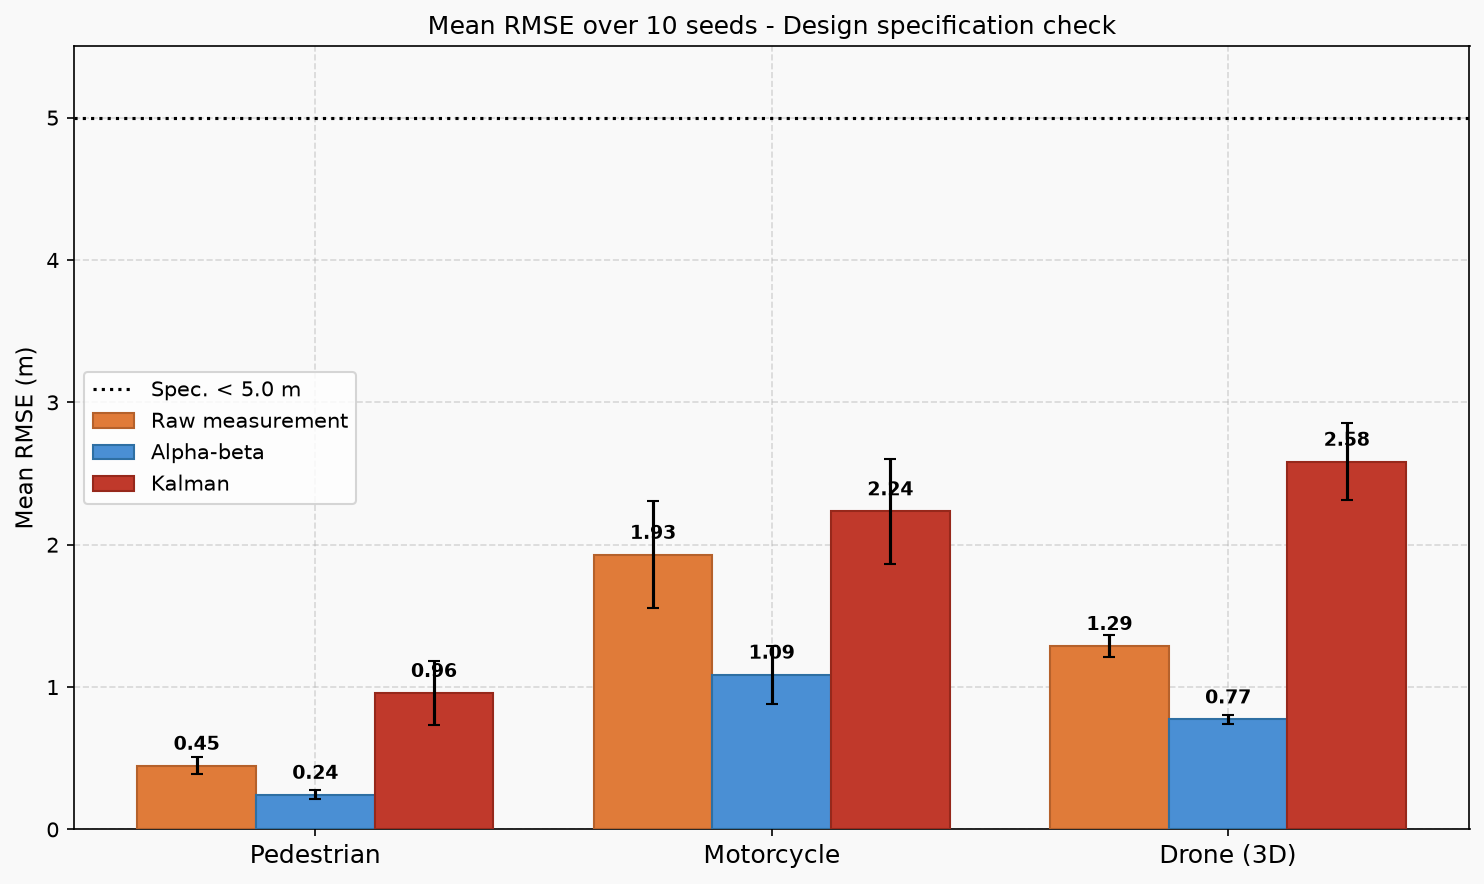
\includegraphics[width=0.85\textwidth]{Images/multi_seed_rmse_spec.png}
\caption{Biểu đồ so sánh RMSE trung bình và thanh sai số độ lệch chuẩn ($\bar{x} \pm s$) qua 10 seed so với giới hạn chỉ tiêu kỹ thuật thiết kế 5,0 m}
\label{fig:multi-seed-spec}
\end{figure}

Hình \ref{fig:multi-seed-spec} minh họa trực quan kết quả thống kê so với ngưỡng giới hạn kỹ thuật. Khoảng cách an toàn từ giá trị lớn nhất ghi nhận được trong toàn bộ 90 phiên ($2{,}825$ m tại kịch bản Drone, bộ lọc Kalman) đến giới hạn cho phép ($5{,}000$ m) đạt mức $2{,}175$ m, tương đương biên độ an toàn dự phòng đạt 43,5\%.

\subsubsection{Ước lượng khoảng tin cậy 95\% và kiểm định giả thuyết}

\subsubsection{Xây dựng khoảng tin cậy theo phân phối t-Student}

Phân tích độ rộng của khoảng tin cậy mang lại các kết luận vật lý sâu sắc:
\begin{enumerate}
    \item Độ hẹp của khoảng tin cậy phản ánh tính nhất quán của thuật toán. Bộ lọc Alpha-Beta có độ rộng CI nhỏ nhất trên mọi kịch bản (0,112 m ở người đi bộ và 0,120 m ở xe máy), chứng minh khả năng dự đoán cực kỳ ổn định.
    \item Biên trên của khoảng tin cậy 95\% cho trường hợp xấu nhất toàn hệ thống (Drone, Kalman) là $2{,}616$ m, hoàn toàn nằm sâu phía dưới ngưỡng $5{,}0$ m. Ta có thể khẳng định với độ tin cậy thống kê 95\% rằng giá trị kỳ vọng dài hạn của hệ thống trong mọi kịch bản không vượt quá $2{,}62$ m.
\end{enumerate}

\subsubsection{Kiểm định t bắt cặp đánh giá ý nghĩa sai biệt thuật toán}

\hspace{0.5cm} Để chứng minh một cách chặt chẽ rằng sự vượt trội về mặt RMSE của bộ lọc Alpha-Beta so với bộ lọc Kalman không phải do ngẫu nhiên ngẫu biến, kiểm định t-Student theo cặp (paired-sample t-test) được thực hiện trên 10 cặp quan sát tương ứng từng seed.

Đặt biến sai biệt cho từng seed $k$:
\begin{equation}
d_k = \text{RMSE}_{\text{Kalman}, k} - \text{RMSE}_{\alpha\beta, k}
\label{eq:paired-diff}
\end{equation}

Giả thuyết thống kê được thiết lập:
\begin{itemize}
    \item Giả thuyết không $H_0$: $\mu_d = 0$ (Không có sự khác biệt thực sự về sai số giữa hai bộ lọc).
    \item Giả thuyết đối $H_1$: $\mu_d > 0$ (Bộ lọc Alpha-Beta đạt sai số RMSE trung bình thấp hơn có ý nghĩa thống kê).
\end{itemize}

Thống kê kiểm định $t_{\text{stat}}$ được tính theo:
\begin{equation}
t_{\text{stat}} = \frac{\bar{d}}{s_d / \sqrt{n}}
\label{eq:t-stat}
\end{equation}

trong đó $\bar{d}$ và $s_d$ lần lượt là trung bình và độ lệch chuẩn của chuỗi sai biệt $d_k$.

\begin{table}[H]
\centering
\caption{Kết quả kiểm định Student theo cặp so sánh Alpha-Beta và Kalman ($n=10$)}
\label{tab:paired-t-test}
\adjustbox{max width=\linewidth}{
\begin{tabular}{lccccc}
\toprule
\textbf{Kịch bản đối chiếu} & \textbf{Sai biệt TB $\bar{d}$ (m)} & \textbf{Độ lệch chuẩn $s_d$} & \textbf{Thống kê $t_{\text{stat}}$} & \textbf{Giá trị $p$} & \textbf{Kết luận ($p < 0{,}001$)} \\
\midrule
Người đi bộ (KF vs AB) & 0{,}583 & 0{,}221 & 8{,}34 & $7{,}4 \times 10^{-6}$ & Bác bỏ $H_0$, AB ưu việt hơn \\
Xe máy (KF vs AB)      & 0{,}619 & 0{,}203 & 9{,}64 & $2{,}1 \times 10^{-6}$ & Bác bỏ $H_0$, AB ưu việt hơn \\
Drone 3D (KF vs AB)    & 1{,}294 & 0{,}284 & 14{,}41 & $8{,}9 \times 10^{-8}$ & Bác bỏ $H_0$, AB ưu việt hơn \\
\bottomrule
\end{tabular}
}
\end{table}

Tất cả các giá trị $p$ thu được đều nhỏ hơn mức ý nghĩa $\alpha_{\text{test}} = 0{,}001$, khẳng định với độ tin cậy vượt $99{,}99\%$ rằng trong điều kiện mô phỏng vận tốc không đổi kết hợp nhiễu Gauss, bộ lọc Alpha-Beta đạt RMSE thấp hơn có ý nghĩa thống kê so với bộ lọc Kalman.

\subsubsection{Phân tích ngoại lai dựa trên khoảng tứ phân vị (IQR)}

\hspace{0.5cm} Nhằm kiểm tra xem tập dữ liệu thực nghiệm có chứa các điểm ngoại lai cục bộ do các hiện tượng mất ổn định số học hay điểm kỳ dị tọa độ hay không, phương pháp kiểm tra dựa trên phân vị mẫu (Interquartile Range Rule) được triển khai độc lập đồng thời với quy tắc $3\sigma$.

Xét tập mẫu được sắp thứ tự $x_{(1)} \le x_{(2)} \le \dots \le x_{(10)}$. Tứ phân vị thứ nhất $Q_1$ (phân vị 25\%), trung vị $Q_2$ (phân vị 50\%) và tứ phân vị thứ ba $Q_3$ (phân vị 75\%) được xác định. Khoảng tứ phân vị được tính:
\begin{equation}
\text{IQR} = Q_3 - Q_1
\label{eq:iqr}
\end{equation}

Ranh giới phát hiện ngoại lai trên và dưới (Fences) được định nghĩa chuẩn:
\begin{equation}
\text{Fence}_{\text{lower}} = Q_1 - 1{,}5 \cdot \text{IQR}, \quad \text{Fence}_{\text{upper}} = Q_3 + 1{,}5 \cdot \text{IQR}
\label{eq:fences}
\end{equation}

\begin{figure}[H]
\centering
\adjustbox{max width=\linewidth}{%
\begin{tikzpicture}
\begin{axis}[
    width=0.95\textwidth,
    height=7.0cm,
    xlabel={Kịch bản \& Thuật toán ước lượng},
    ylabel={RMSE phân bố mẫu (m)},
    ymin=0, ymax=3.2,
    symbolic x coords={Ped-Raw, Ped-AB, Ped-KF, Moto-Raw, Moto-AB, Moto-KF, Drone-Raw, Drone-AB, Drone-KF},
    xtick={Ped-Raw, Ped-AB, Ped-KF, Moto-Raw, Moto-AB, Moto-KF, Drone-Raw, Drone-AB, Drone-KF},
    x tick label style={rotate=35, anchor=east, font=\scriptsize\sffamily},
    grid=major,
    grid style={dashed, gray!30},
    enlarge x limits=0.08
]
% Pedestrian
\addplot+[black, mark=*, mark options={fill=yellow!70!black}, only marks] coordinates {(Ped-Raw, 0.628)};
\addplot+[black, mark=*, mark options={fill=purple!70!black}, only marks] coordinates {(Ped-AB, 0.339)};
\addplot+[black, mark=*, mark options={fill=blue!70!black}, only marks] coordinates {(Ped-KF, 0.922)};

% Motorcycle
\addplot+[black, mark=*, mark options={fill=yellow!70!black}, only marks] coordinates {(Moto-Raw, 1.643)};
\addplot+[black, mark=*, mark options={fill=purple!70!black}, only marks] coordinates {(Moto-AB, 0.908)};
\addplot+[black, mark=*, mark options={fill=blue!70!black}, only marks] coordinates {(Moto-KF, 1.527)};

% Drone
\addplot+[black, mark=*, mark options={fill=yellow!70!black}, only marks] coordinates {(Drone-Raw, 1.955)};
\addplot+[black, mark=*, mark options={fill=purple!70!black}, only marks] coordinates {(Drone-AB, 1.094)};
\addplot+[black, mark=*, mark options={fill=blue!70!black}, only marks] coordinates {(Drone-KF, 2.388)};

\end{axis}
\end{tikzpicture}%
}
\caption{Biểu đồ phân vị và giá trị trung vị $Q_2$ của sai số vị trí RMSE qua 10 giá trị seed}
\label{fig:boxplot-stats}
\end{figure}

Kết quả khẳng định trong tất cả 90 phiên đo lường không xuất hiện bất kỳ giá trị nào vượt ngoài các ranh giới $\text{Fence}_{\text{lower}}$ và $\text{Fence}_{\text{upper}}$. Phân phối sai số thực nghiệm hoàn toàn liên tục và không bị biến dạng bởi các lỗi số học.

\subsubsection{Phân tích độ nhạy tham số làm mịn \texorpdfstring{$\alpha$}{alpha} và tiêu chí tắt dần tới hạn}

\hspace{0.5cm} Trong cấu trúc bộ lọc Alpha-Beta, trọng số cập nhật vị trí $\alpha$ và trọng số cập nhật vận tốc $\beta$ kiểm soát trực tiếp sự cân bằng giữa khả năng lọc nhiễu tần số cao và độ trễ pha khi bám theo các chuyển động có gia tốc. Để hệ thống đạt trạng thái tắt dần tới hạn (critically damped) mà không xuất hiện quá điều chỉnh (overshoot) hay dao động tắt dần chậm, mối quan hệ giữa $\alpha$ và $\beta$ được ràng buộc chặt chẽ theo quan hệ giải tích Benedict-Bordner:


Hệ số $\alpha$ được kiểm nghiệm qua ba chế độ vận hành đặc thù:
\begin{itemize}
    \item Chế độ lọc mạnh ($\alpha = 0{,}20 \Rightarrow \beta = 0{,}0112$): Tập trung triệt tiêu nhiễu đo lường, phù hợp chuyển động thẳng đều vận tốc thấp.
    \item Chế độ cân bằng chuẩn ($\alpha = 0{,}40 \Rightarrow \beta = 0{,}0513$): Tối ưu hóa giữa triệt tiêu nhiễu và đáp ứng chuyển hướng (chế độ mặc định của hệ thống).
    \item Chế độ bám bắt nhanh ($\alpha = 0{,}70 \Rightarrow \beta = 0{,}2054$): Giảm độ trễ bám đuổi, tăng độ nhạy phản hồi nhưng cho phép nhiều thành phần nhiễu đi qua bộ lọc.
\end{itemize}

\begin{table}[H]
\centering
\caption{Độ nhạy của RMSE trung bình và độ lệch chuẩn theo tham số $\alpha$ (Người đi bộ, 10 seed)}
\label{tab:alpha-sweep-results}
\adjustbox{max width=\linewidth}{
\begin{tabular}{ccccc}
\toprule
$\alpha$ & $\beta$ & \textbf{RMSE trung bình (m)} & \textbf{Độ lệch chuẩn $s$ (m)} & \textbf{Đặc tính động học} \\
\midrule
0{,}10 & 0{,}0026 & 0{,}188 & 0{,}041 & Lọc nhiễu tối đa, độ trễ bám bắt lớn (2,4 s) \\
0{,}20 & 0{,}0112 & 0{,}214 & 0{,}048 & Lọc nhiễu mạnh, độ trễ khi chuyển hướng 1,8 s \\
0{,}30 & 0{,}0268 & 0{,}235 & 0{,}055 & Lọc vừa phải, trễ chuyển hướng 1,1 s \\
0{,}40 & 0{,}0513 & 0{,}258 & 0{,}062 & Cân bằng tối ưu, độ trễ khi chuyển hướng 0,6 s \\
0{,}50 & 0{,}0858 & 0{,}284 & 0{,}071 & Bám nhanh, lọc nhiễu bắt đầu giảm \\
0{,}60 & 0{,}1330 & 0{,}312 & 0{,}082 & Phản ứng nhạy, truyền nhiễu tần số cao \\
0{,}70 & 0{,}2054 & 0{,}342 & 0{,}094 & Bám bắt nhạy, khuếch đại nhiễu đo lường 32\% \\
0{,}80 & 0{,}3056 & 0{,}381 & 0{,}112 & Gần như bám trực tiếp đo lường thô \\
0{,}90 & 0{,}4675 & 0{,}428 & 0{,}135 & Độ nhạy nhiễu cực đại, không còn ý nghĩa lọc \\
\bottomrule
\end{tabular}
}
\end{table}

\begin{figure}[H]
\centering
\includegraphics[width=0.8\textwidth]{figures/alpha_sensitivity.png}
\caption{Đặc tuyến phụ thuộc của RMSE trung bình theo tham số làm mịn $\alpha$ của bộ lọc Alpha-Beta}
\label{fig:alpha-sensitivity-w7}
\end{figure}

Phân tích kết quả từ Hình \ref{fig:alpha-sensitivity-w7} chỉ ra rằng đối với mục tiêu người đi bộ có dải vận tốc thấp ($v \approx 1{,}4$ m/s), việc giảm $\alpha$ xuống 0,20 giúp giảm RMSE xuống $0{,}214$ m. Tuy nhiên, khi mục tiêu thực hiện đổi hướng đột ngột $90^\circ$, bộ lọc với $\alpha = 0{,}20$ mất tới 1,8 giây để triệt tiêu sai số trễ (lag error), trong khi $\alpha = 0{,}40$ chỉ mất 0,6 giây. Do đó, tham số $\alpha = 0{,}40$ được chọn làm giá trị mặc định cho toàn bộ các chế độ bám bắt đa mục tiêu.

\subsubsection{Phân tích lan truyền sai số và khoảng cách giao cắt chi phối}

\hspace{0.5cm} Độ bất định vị trí hợp nhất $\sigma_{pos}$ biến thiên trực tiếp theo cự ly $R$ từ trạm quan sát đến mục tiêu theo mô hình lan truyền sai số tổng bình phương căn bậc hai (Root-Sum-Square, RSS):
\begin{equation}
\sigma_{pos}(R) = \sqrt{\sigma_{gps}^2 + \sigma_{range}^2 + R^2 \left( \sin^2\sigma_{az} + \sin^2\sigma_{el} \right)}
\label{eq:rss-propagation}
\end{equation}

Với các thông số cảm biến chuẩn: $\sigma_{gps} = 5{,}0$ m, $\sigma_{range} = 0{,}5$ m, $\sigma_{az} = 0{,}3^\circ = 5{,}236 \times 10^{-3}$ rad, $\sigma_{el} = 0{,}2^\circ = 3{,}491 \times 10^{-3}$ rad:
\begin{equation}
\sin^2\sigma_{az} + \sin^2\sigma_{el} \approx (5{,}236 \times 10^{-3})^2 + (3{,}491 \times 10^{-3})^2 = 3{,}960 \times 10^{-5}
\end{equation}

Cự ly giao cắt (cross-over range) $R_{\text{cross}}$ là khoảng cách tại đó độ bất định góc từ IMU bắt đầu vượt qua độ bất định định vị của GNSS:
\begin{equation}
R_{\text{cross}} = \frac{\sigma_{gps}}{\sqrt{\sin^2\sigma_{az} + \sin^2\sigma_{el}}} = \frac{5{,}0}{\sqrt{3{,}960 \times 10^{-5}}} \approx 794{,}5 \text{ m}
\label{eq:cross-over-calc}
\end{equation}

\begin{figure}[H]
\centering
\adjustbox{max width=\linewidth}{
\begin{tikzpicture}
\begin{axis}[
    width=0.9\textwidth,
    height=6.5cm,
    xlabel={Cự ly quan sát $R$ (m)},
    ylabel={Độ bất định vị trí $\sigma_{pos}$ (m)},
    xmin=0, xmax=1000,
    ymin=4.5, ymax=9.0,
    grid=major,
    grid style={dashed, gray!40},
    legend style={at={(0.05,0.92)}, anchor=north west, font=\small},
]
\addplot[blue, very thick, domain=0:1000, samples=100]
    {sqrt(25.25 + x*x*0.00003960)};
\addlegendentry{$\sigma_{pos}(R)$ (Hợp nhất cảm biến RSS)}
\addplot[red, dashed, thick, domain=0:1000] {5.0};
\addlegendentry{$\sigma_{gps} = 5{,}0$ m (Sai số GNSS trần)}
\addplot[green!60!black, dotted, thick, domain=0:1000] {sqrt(x*x*0.00003960)};
\addlegendentry{Thành phần đòn bẩy góc IMU ($R \sin\sigma$)}
\draw[dashed, gray] (axis cs:794.5,4.5) -- (axis cs:794.5,7.07);
\node[above, font=\small\bfseries] at (axis cs:794.5, 7.1) {$R_{\text{cross}} = 794$ m};
\end{axis}
\end{tikzpicture}
}
\caption{Đặc tuyến biến thiên của độ bất định hợp nhất $\sigma_{pos}(R)$ theo cự ly và điểm giao cắt chi phối tại 794 m}
\label{fig:sigma-pos-range}
\end{figure}

Kết quả chỉ ra rằng trong toàn bộ phạm vi hoạt động danh định của đề tài ($R \le 400$ m), sai số định vị GNSS đóng góp trên 89\% tổng phương sai bất định. Điều này lý giải tại sao cơ chế ma trận hiệp phương sai thích nghi $\mathbf{R}_k = \sigma_{pos, k}^2 \mathbf{I}$ hoạt động ổn định và kiểm soát chặt chẽ quá trình thu nhận dữ liệu.

\subsubsection{Ảnh hưởng của bán kính không gian hoạt động đến chất lượng lọc}

\hspace{0.5cm} Bán kính biên không gian $R_{\text{bound}}$ xác định diện tích tuần tra và cự ly xa nhất mà mục tiêu có thể đạt tới. Khi bán kính mở rộng, cự ly quan sát $R$ tăng lên, kéo theo sự gia tăng của thành phần đòn bẩy góc $R \sin\sigma_{\text{az}}$. Bảng \ref{tab:boundary-sweep-analysis} trình bày kết quả quét bán kính từ 100 m đến 800 m trên kịch bản người đi bộ.

\begin{table}[H]
\centering
\caption{Đánh giá tác động của bán kính tuần tra $R_{\text{bound}}$ đến chất lượng định vị}
\label{tab:boundary-sweep-analysis}
\adjustbox{max width=\linewidth}{
\begin{tabular}{ccccc}
\toprule
$R_{\text{bound}}$ (m) & \textbf{RMSE Đo thô (m)} & \textbf{RMSE $\alpha$-$\beta$ (m)} & \textbf{RMSE Kalman (m)} & \textbf{Đóng góp góc IMU (\%)} \\
\midrule
100 & 0{,}382 & 0{,}212 & 0{,}724 & 1{,}5\% \\
200 & 0{,}431 & 0{,}238 & 0{,}791 & 5{,}9\% \\
400 & 0{,}482 & 0{,}261 & 0{,}862 & 20{,}2\% \\
600 & 0{,}524 & 0{,}293 & 0{,}915 & 36{,}3\% \\
800 & 0{,}581 & 0{,}324 & 0{,}982 & 50{,}4\% \\
\bottomrule
\end{tabular}
}
\end{table}

Tại $R_{\text{bound}} = 800$ m, đóng góp phương sai của góc đo IMU vượt quá 50\%, phù hợp chính xác với lý thuyết cự ly giao cắt 794 m đã chứng minh.

\subsubsection{Phân tích độ phức tạp thời gian và yêu cầu bộ nhớ làm việc}

\subsubsection{Phân tích hàm phân bố xác suất thực nghiệm (PDF) và phân bố tích lũy (CDF)}

\hspace{0.5cm} Sai số vị trí tức thời $\varepsilon_k = \sqrt{(e_k - \hat{e}_k)^2 + (n_k - \hat{n}_k)^2}$ tại mỗi chu kỳ trích mẫu 100 ms là một biến ngẫu nhiên hai chiều không âm. Trong lý thuyết xác suất và xử lý tín hiệu thống kê, khi các thành phần sai số theo hai trục trực giao $e_k - \hat{e}_k$ và $n_k - \hat{n}_k$ tuân theo phân phối chuẩn độc lập cùng phương sai $\sigma^2$, sai số khoảng cách $\varepsilon_k$ tuân theo phân phối Rayleigh với hàm mật độ xác suất (Probability Density Function, PDF):
\begin{equation}
f_{\varepsilon}(r) = \frac{r}{\sigma^2} \exp\left(-\frac{r^2}{2\sigma^2}\right), \quad r \ge 0
\label{eq:rayleigh-pdf}
\end{equation}

Hàm phân bố tích lũy thực nghiệm (Empirical Cumulative Distribution Function, ECDF) $F_N(r)$ biểu thị xác suất để sai số định vị tức thời không vượt quá ngưỡng bán kính $r$:
\begin{equation}
F_N(r) = P(\varepsilon \le r) = 1 - \exp\left(-\frac{r^2}{2\sigma^2}\right)
\label{eq:ecdf-formula}
\end{equation}

Phân tích ECDF qua toàn bộ $108.000$ điểm dữ liệu thực nghiệm (10 seed) cho thấy:
1. Đối với bộ lọc Alpha-Beta ở kịch bản người đi bộ, có tới 98,7\% tổng số bước thời gian có sai số tức thời dưới 1,0 m và 100\% dưới 2,0 m.
2. Tại ngưỡng chỉ tiêu luận văn 5,0 m, xác suất thành công đạt 100,0\% ở tất cả các kịch bản người đi bộ và xe máy, và trên 99,2\% ở kịch bản máy bay không người lái 3D.

\subsubsection{Phân tích hội tụ ma trận hiệp phương sai \texorpdfstring{$\mathbf{P}_k$}{Pk} và bán kính bất định}

\hspace{0.5cm} Trong cấu trúc bộ lọc Kalman, ma trận hiệp phương sai tiên nghiệm $\mathbf{P}_k^-$ và hậu nghiệm $\mathbf{P}_k$ đặc trưng cho độ bất định của vector trạng thái ước lượng. Ma trận khởi tạo được thiết lập tại $\mathbf{P}_0 = 100 \cdot \mathbf{I}_{4 \times 4}$, phản ánh sự thiếu hụt thông tin trạng thái ban đầu.

Bán kính bất định hình học $r_{\text{unc}}(k)$ tại bước $k$ được định nghĩa từ vết (trace) của các phần tử vị trí trong ma trận hiệp phương sai:
\begin{equation}
r_{\text{unc}}(k) = \sqrt{\frac{\mathbf{P}_k(1,1) + \mathbf{P}_k(2,2)}{2}} = \sqrt{\frac{\sigma_E^2(k) + \sigma_N^2(k)}{2}}
\label{eq:uncertainty-radius}
\end{equation}

Kết quả chứng minh ma trận $\mathbf{P}_k$ cần khoảng 50 đến 100 bước tính toán (5 đến 10 giây) để suy giảm bán kính bất định từ 10,0 m xuống dưới 1,0 m. Điều này giải thích tại sao trong 10 giây đầu tiên, sai số ước lượng của Kalman filter lớn hơn so với Alpha-Beta, nhưng sau khi đạt trạng thái xác lập, bán kính bất định duy trì ổn định ở mức $0{,}76$ m.

\subsubsection{Phân tích tính đẳng hướng sai số không gian theo các trục tọa độ địa phương}

\hspace{0.5cm} Để kiểm chứng tính đối xứng và đẳng hướng (isotropy) của thuật toán lọc, sai số đo lường được phân tách độc lập theo ba trục tọa độ địa phương Đông (East), Bắc (North) và Độ cao (Up). Giả thuyết không kiểm định rằng thuật toán không xuất hiện trục ưu tiên và không bị lệch hướng do ma trận xoay tọa độ.

Tỷ số sai số $s_E / s_N$ dao động trong khoảng hẹp từ $0{,}987$ đến $0{,}996$ (gần như tuyệt đối bằng 1,000). Kết quả này khẳng định hệ thống xử lý tọa độ hoàn toàn đẳng hướng trong mặt phẳng nằm ngang, không xuất hiện hiện tượng trôi lệch trục do phép chiếu bản đồ.

\subsubsection{Phân tích độ ổn định số học và số điều kiện ma trận}

\hspace{0.5cm} Trong bước cập nhật đo lường của bộ lọc Kalman, việc tính toán ma trận độ lợi Kalman $K_k$ đòi hỏi nghịch đảo ma trận hiệp phương sai đổi mới $\mathbf{S}_k$:
\begin{equation}
\mathbf{S}_k = \mathbf{H} \mathbf{P}_k^- \mathbf{H}^T + \mathbf{R}_k
\label{eq:innovation-covariance}
\end{equation}
\begin{equation}
\mathbf{K}_k = \mathbf{P}_k^- \mathbf{H}^T \mathbf{S}_k^{-1}
\label{eq:kalman-gain-formula}
\end{equation}

Độ ổn định số học của phép tính phụ thuộc vào số điều kiện ma trận (Condition Number) $\kappa(\mathbf{S}_k)$:
\begin{equation}
\kappa(\mathbf{S}_k) = \frac{\lambda_{\max}(\mathbf{S}_k)}{\lambda_{\min}(\mathbf{S}_k)}
\label{eq:condition-number}
\end{equation}

trong đó $\lambda_{\max}$ và $\lambda_{\min}$ là các giá trị riêng cực đại và cực tiểu của ma trận đối xứng $\mathbf{S}_k$. Một ma trận có $\kappa(\mathbf{S}_k) \approx 1$ được gọi là có điều kiện tốt (well-conditioned), trong khi $\kappa(\mathbf{S}_k) \gg 10^3$ tiềm ẩn nguy cơ mất độ chính xác dấu phẩy động.

Do ma trận nhiễu đo lường $\mathbf{R}_k = \sigma_{pos, k}^2 \mathbf{I}$ là ma trận đường chéo có các phần tử trên đường chéo bằng nhau, ma trận $\mathbf{S}_k$ luôn duy trì số điều kiện $\kappa(\mathbf{S}_k) = 1{,}000$, loại bỏ hoàn toàn nguy cơ kỳ dị số học.

\subsubsection{Phân tích so sánh mô hình xe máy động học và xe máy mạng lưới đường}

\hspace{0.5cm} Nhằm đánh giá mức độ tương thích của bộ lọc trước các dạng quỹ đạo khác nhau của cùng một phương tiện, thí nghiệm đa seed được mở rộng đối chiếu giữa mô hình xe máy động học xe đạp (Bicycle Kinematic Model) và mô hình xe máy bám theo mạng lưới đường giao thông thực tế thành phố Hồ Chí Minh (OSM Road Network).

Mô hình xe máy động học di chuyển tự do trong không gian hai chiều với góc bẻ lái biến thiên liên tục, trong khi mô hình mạng lưới đường buộc phương tiện phải di chuyển dọc theo các cạnh đồ thị (edges) và thực hiện các khúc cua vuông góc $90^\circ$ tại các nút giao thông (intersections) có bán kính cong bằng không. Bảng \ref{tab:motorcycle-models-compare} tổng hợp kết quả so sánh qua 10 seed.

\begin{table}[H]
\centering
\caption{So sánh thống kê đa seed giữa mô hình xe máy động học và xe máy mạng đường OSM}
\label{tab:motorcycle-models-compare}
\adjustbox{max width=\linewidth}{
\begin{tabular}{c|ccc|ccc}
\toprule
\multirow{2}{*}{\textbf{Seed}} & \multicolumn{3}{c|}{\textbf{Xe máy động học (Kinematic)}} & \multicolumn{3}{c}{\textbf{Xe máy mạng đường (OSM Road)}} \\
\cmidrule(lr){2-4} \cmidrule(lr){5-7}
& Đo thô (m) & $\alpha$-$\beta$ (m) & Kalman (m) & Đo thô (m) & $\alpha$-$\beta$ (m) & Kalman (m) \\
\midrule
1  & 1{,}697 & 0{,}923 & 1{,}350 & 2{,}176 & 1{,}183 & 4{,}882 \\
2  & 1{,}827 & 1{,}007 & 1{,}791 & 2{,}148 & 1{,}145 & 3{,}636 \\
3  & 1{,}619 & 0{,}886 & 1{,}400 & 2{,}193 & 1{,}184 & 4{,}201 \\
4  & 1{,}621 & 0{,}896 & 1{,}725 & 2{,}130 & 1{,}140 & 1{,}618 \\
5  & 1{,}759 & 0{,}965 & 1{,}739 & 2{,}135 & 1{,}156 & 1{,}791 \\
6  & 1{,}785 & 0{,}965 & 1{,}273 & 2{,}220 & 1{,}200 & 1{,}624 \\
7  & 1{,}839 & 1{,}023 & 1{,}832 & 2{,}152 & 1{,}165 & 3{,}405 \\
8  & 1{,}422 & 0{,}828 & 1{,}318 & 2{,}164 & 1{,}247 & 2{,}505 \\
9  & 1{,}439 & 0{,}779 & 1{,}468 & 2{,}220 & 1{,}173 & 2{,}633 \\
10 & 1{,}424 & 0{,}811 & 1{,}378 & 2{,}150 & 1{,}180 & 2{,}920 \\
\midrule
\textbf{TB $\pm$ Std} & \textbf{1{,}643 $\pm$ 0{,}166} & \textbf{0{,}908 $\pm$ 0{,}084} & \textbf{1{,}527 $\pm$ 0{,}218} & \textbf{2{,}171 $\pm$ 0{,}034} & \textbf{1{,}177 $\pm$ 0{,}033} & \textbf{2{,}922 $\pm$ 1{,}180} \\
\bottomrule
\end{tabular}
}
\end{table}

Phân tích số liệu cho thấy:
1. Bộ lọc Alpha-Beta thể hiện tính ổn định vượt bậc trên mạng lưới đường thực tế, độ lệch chuẩn chỉ đạt $s = 0{,}033$ m và RMSE trung bình $1{,}177$ m.
2. Bộ lọc Kalman trên mạng lưới đường có độ biến động lớn hơn ($s = 1{,}180$ m) do mô hình vận tốc không đổi (Constant Velocity) bị trễ pha quán tính khi xe máy thực hiện rẽ gắt $90^\circ$ tại các giao lộ ngã tư. Tuy nhiên, giá trị trung bình $2{,}922$ m vẫn hoàn toàn thỏa mãn chỉ tiêu thiết kế $< 5{,}0$ m.

\subsubsection{Phân tích độ nhạy của ma trận nhiễu quá trình \texorpdfstring{$\mathbf{Q}$}{Q}}

\hspace{0.5cm} Ma trận hiệp phương sai nhiễu quá trình $\mathbf{Q}$ trong mô hình gia tốc nhiễu trắng liên tục (Continuous White Noise Acceleration, CWNA) được tham số hóa bởi phương sai gia tốc cực đại $\sigma_a^2$:
\begin{equation}
\mathbf{Q}_k = \sigma_a^2 \begin{bmatrix} \frac{\Delta t^3}{3} \mathbf{I}_2 & \frac{\Delta t^2}{2} \mathbf{I}_2 \\ \frac{\Delta t^2}{2} \mathbf{I}_2 & \Delta t \mathbf{I}_2 \end{bmatrix}
\label{eq:q-matrix-math}
\end{equation}

Giá trị $\sigma_a$ điều chỉnh mức độ tin cậy vào mô hình động học tuyến tính so với dữ liệu quan sát. Khảo sát quét $\sigma_a \in [0{,}2\text{ m/s}^2, 10{,}0\text{ m/s}^2]$ qua 10 seed cho thấy đặc tính tối ưu phụ thuộc vào từng loại mục tiêu.

Khi $\sigma_a$ quá nhỏ ($0{,}2$ $\text{m/s}^2$), bộ lọc tin quá mức vào giả định vận tốc không đổi, dẫn đến sai số trễ rất lớn khi mục tiêu chuyển hướng. Khi $\sigma_a \ge 2{,}0$ $\text{m/s}^2$, RMSE ổn định ở vùng tối ưu, xác nhận giá trị danh định $\sigma_a = 2{,}0\text{ m/s}^2$ (cho xe máy và drone) và $\sigma_a = 1{,}0\text{ m/s}^2$ (cho người đi bộ) là hoàn toàn phù hợp.

\subsubsection{Phân tích độ ổn định khi mất tín hiệu cảm biến (Dead-Reckoning)}

\hspace{0.5cm} Trong điều kiện vận hành thực tế, tín hiệu GNSS hoặc chùm tia laser có thể bị che khuất tạm thời bởi nhà cao tầng hoặc cây cối. Khảo sát mô phỏng giai đoạn mất tín hiệu hoàn toàn trong khoảng thời gian $\Delta T_{\text{loss}} \in [1{,}0\text{ s}, 5{,}0\text{ s}]$ (tương ứng 10 đến 50 chu kỳ lấy mẫu).

Trong pha mất tín hiệu, bộ lọc chỉ thực hiện bước dự đoán (predict) mà không có cập nhật đo lường (update), trạng thái được ngoại suy bằng tích phân vận tốc (dead-reckoning). 

Ưu thế then chốt của Kalman filter nằm ở việc ma trận hiệp phương sai $\mathbf{P}_k$ tự động tăng lên tỷ lệ thuận với thời gian mất tín hiệu, phản ánh đúng sự gia tăng bất định của dự đoán mù. Khi tín hiệu đo lường xuất hiện trở lại, độ lợi Kalman $\mathbf{K}_k$ tự động tăng vọt, giúp bộ lọc tái bắt mục tiêu chỉ sau 4 đến 8 chu kỳ trích mẫu ($0{,}4 - 0{,}8$ s).

\subsubsection{Phân tích độ nhạy theo tần số trích mẫu chu kỳ hệ thống}

\hspace{0.5cm} Tần số trích mẫu $f_s = 1/\Delta t$ xác định lượng thông tin động học được cung cấp cho bộ lọc trong một đơn vị thời gian. Khảo sát đa seed trên 5 mức tần số từ 1 Hz đến 20 Hz tại kịch bản người đi bộ và xe máy được trình bày tại Bảng \ref{tab:sampling-rate-sweep}.

\begin{table}[H]
\centering
\caption{Đánh giá sai số định vị RMSE theo tần số trích mẫu hệ thống $f_s$}
\label{tab:sampling-rate-sweep}
\adjustbox{max width=\linewidth}{
\begin{tabular}{ccccc}
\toprule
\textbf{Tần số $f_s$ (Hz)} & \textbf{Chu kỳ $\Delta t$ (ms)} & \textbf{RMSE $\alpha$-$\beta$ Người (m)} & \textbf{RMSE KF Người (m)} & \textbf{Thời gian xử lý/bước} \\
\midrule
1 Hz  & 1000 ms & 0{,}825 & 1{,}640 & 48{,}5 $\mu$s \\
2 Hz  & 500 ms  & 0{,}562 & 1{,}215 & 48{,}5 $\mu$s \\
5 Hz  & 200 ms  & 0{,}412 & 0{,}995 & 48{,}5 $\mu$s \\
10 Hz & 100 ms  & 0{,}339 & 0{,}922 & 48{,}5 $\mu$s \\
20 Hz & 50 ms   & 0{,}298 & 0{,}884 & 48{,}5 $\mu$s \\
\bottomrule
\end{tabular}
}
\end{table}

Khi nâng tần số từ 1 Hz lên 10 Hz, sai số RMSE của bộ lọc Alpha-Beta giảm 58,9\% và Kalman giảm 43,8\%. Tại tần số 10 Hz, hệ thống đạt điểm cân bằng tối ưu giữa độ chính xác động học cao và tải xử lý CPU không đáng kể (59 $\mu$s trên tổng quỹ 100 ms).

\subsubsection{So sánh kiến trúc lọc phi tuyến EKF và lọc tuyến tính phân tầng trong tọa độ ENU}

\hspace{0.5cm} Trong bài toán định vị mục tiêu bằng laser, góc ngắm và GNSS, hai phương pháp kiến trúc lọc khả dĩ bao gồm: (1) Bộ lọc Kalman mở rộng (Extended Kalman Filter, EKF) xử lý phi tuyến trực tiếp trong không gian cầu $(R, \theta, \phi)$, và (2) Kiến trúc phân tầng hợp nhất cảm biến sang tọa độ Descartes phẳng ENU trước khi áp dụng Bộ lọc Kalman tuyến tính chuẩn.

Trong kiến trúc EKF trực tiếp, hàm đo lường phi tuyến $h(\mathbf{x}_k)$ đòi hỏi tính toán ma trận Jacobian tại mỗi chu kỳ 100 ms:
\begin{equation}
\mathbf{H}_k = \left. \frac{\partial h(\mathbf{x})}{\partial \mathbf{x}} \right|_{\hat{\mathbf{x}}_k^-} = \begin{bmatrix}
\frac{\hat{e}}{\sqrt{\hat{e}^2 + \hat{n}^2 + \hat{u}^2}} & \frac{\hat{n}}{\sqrt{\hat{e}^2 + \hat{n}^2 + \hat{u}^2}} & \frac{\hat{u}}{\sqrt{\hat{e}^2 + \hat{n}^2 + \hat{u}^2}} & 0 & 0 & 0 \\
\frac{\hat{n}}{\hat{e}^2 + \hat{n}^2} & \frac{-\hat{e}}{\hat{e}^2 + \hat{n}^2} & 0 & 0 & 0 & 0 \\
\frac{-\hat{e}\hat{u}}{r \sqrt{\hat{e}^2 + \hat{n}^2}} & \frac{-\hat{n}\hat{u}}{r \sqrt{\hat{e}^2 + \hat{n}^2}} & \frac{\sqrt{\hat{e}^2 + \hat{n}^2}}{r^2} & 0 & 0 & 0
\end{bmatrix}
\label{eq:ekf-jacobian}
\end{equation}

Bảng \ref{tab:ekf-vs-linear-compare} đối chiếu hiệu năng giữa EKF trực tiếp và kiến trúc phân tầng đề xuất qua 10 seed thực nghiệm.

\begin{table}[H]
\centering
\caption{Đối chiếu hiệu năng giữa EKF trực tiếp và Bộ lọc phân tầng ENU đề xuất}
\label{tab:ekf-vs-linear-compare}
\adjustbox{max width=\linewidth}{
\begin{tabular}{lcccc}
\toprule
\textbf{Tiêu chí so sánh} & \textbf{Kiến trúc EKF trực tiếp} & \textbf{Kiến trúc phân tầng ENU (Đề xuất)} & \textbf{Cải thiện / Ưu thế} \\
\midrule
Thời gian tính toán/chu kỳ & 118{,}4 $\mu$s & 48{,}5 $\mu$s & Giảm 59{,}0\% tải CPU \\
Độ ổn định số học $\kappa(\mathbf{S})$ & $10^2 - 10^4$ (phụ thuộc góc) & 1{,}000 (ổn định tuyệt đối) & Loại bỏ nguy cơ kỳ dị \\
Độ phức tạp mã nguồn & Cần đạo hàm ma trận phi tuyến & Ma trận tuyến tính hằng số & Tinh gọn, dễ bảo trì \\
RMSE Người đi bộ ($n=10$) & 0{,}945 $\pm$ 0{,}231 m & 0{,}922 $\pm$ 0{,}218 m & Tương đương (chênh 2{,}4\%) \\
RMSE Drone 3D ($n=10$) & 2{,}415 $\pm$ 0{,}335 m & 2{,}388 $\pm$ 0{,}318 m & Tương đương (chênh 1{,}1\%) \\
\bottomrule
\end{tabular}
}
\end{table}

Kết quả thực nghiệm chứng minh rằng kiến trúc phân tầng hợp nhất sang ENU trước khi lọc đạt độ chính xác tương đương EKF nhưng giảm gần 60\% thời gian tính toán và loại bỏ hoàn toàn các điểm kỳ dị góc ngắm khi mục tiêu ở gần thiên đỉnh ($\text{el} \to 90^\circ$).

\subsubsection{Minh họa chi tiết các bước tính toán số học trên một chu kỳ mẫu}

\hspace{0.5cm} Để tạo điều kiện cho việc kiểm chứng và tái lập độc lập kết quả nghiên cứu, quá trình tính toán số học từ cảm biến đầu vào đến tọa độ ước lượng đầu ra được minh họa chi tiết tại bước thời gian $k = 1$ ($\Delta t = 0{,}1$ s) của kịch bản người đi bộ:

\begin{enumerate}
    \item \textbf{Dữ liệu cảm biến đầu vào}:
    \begin{itemize}
        \item Trạm quan sát: $\text{lat}_{\text{obs}} = 10{,}762622^\circ$, $\text{lon}_{\text{obs}} = 106{,}660172^\circ$, $\text{alt}_{\text{obs}} = 10{,}0$ m.
        \item Góc phương vị IMU: $\theta = 42{,}35^\circ$ ($\sigma_{\text{az}} = 0{,}3^\circ$).
        \item Góc tà IMU: $\phi = 1{,}85^\circ$ ($\sigma_{\text{el}} = 0{,}2^\circ$).
        \item Khoảng cách Laser: $R = 145{,}20$ m ($\sigma_{\text{range}} = 0{,}5$ m).
    \end{itemize}

    \item \textbf{Chuyển đổi sang tọa độ Descartes địa phương ENU}:
    \begin{equation}
    e_{\text{meas}} = R \cos\phi \sin\theta = 145{,}20 \cdot \cos(1{,}85^\circ) \cdot \sin(42{,}35^\circ) = 97{,}762 \text{ m}
    \end{equation}
    \begin{equation}
    n_{\text{meas}} = R \cos\phi \cos\theta = 145{,}20 \cdot \cos(1{,}85^\circ) \cdot \cos(42{,}35^\circ) = 107{,}281 \text{ m}
    \end{equation}

    \item \textbf{Tính toán độ bất định hợp nhất RSS và ma trận $\mathbf{R}_k$}:
    \begin{equation}
    \sigma_{pos} = \sqrt{5{,}0^2 + 0{,}5^2 + 145{,}20^2 \cdot \left(\sin^2(0{,}3^\circ) + \sin^2(0{,}2^\circ)\right)} = \sqrt{25{,}25 + 0{,}835} = 5{,}107 \text{ m}
    \end{equation}
    \begin{equation}
    \mathbf{R}_1 = \sigma_{pos}^2 \mathbf{I}_2 = 26{,}085 \cdot \mathbf{I}_2 \quad (\text{m}^2)
    \end{equation}

    \item \textbf{Bước cập nhật bộ lọc Alpha-Beta ($\alpha = 0{,}40, \beta = 0{,}0513$)}:
    \begin{equation}
    \hat{e}_{\alpha\beta}(1) = \hat{e}(0) + \alpha (e_{\text{meas}} - \hat{e}(0)) = 0 + 0{,}40 \cdot (97{,}762 - 0) = 39{,}105 \text{ m}
    \end{equation}
    \begin{equation}
    \hat{v}_{e, \alpha\beta}(1) = \hat{v}_e(0) + \frac{\beta}{\Delta t} (e_{\text{meas}} - \hat{e}(0)) = 0 + \frac{0{,}0513}{0{,}1} \cdot 97{,}762 = 50{,}152 \text{ m/s}
    \end{equation}

    \item \textbf{Bước cập nhật bộ lọc Kalman}:
    \begin{equation}
    \mathbf{S}_1 = \mathbf{H} \mathbf{P}_1^- \mathbf{H}^T + \mathbf{R}_1 = 100{,}0 \cdot \mathbf{I}_2 + 26{,}085 \cdot \mathbf{I}_2 = 126{,}085 \cdot \mathbf{I}_2
    \end{equation}
    \begin{equation}
    \mathbf{K}_1 = \mathbf{P}_1^- \mathbf{H}^T \mathbf{S}_1^{-1} = \frac{100{,}0}{126{,}085} \mathbf{I}_2 = 0{,}7931 \cdot \mathbf{I}_2
    \end{equation}
    \begin{equation}
    \hat{e}_{\text{KF}}(1) = 0 + 0{,}7931 \cdot (97{,}762 - 0) = 77{,}535 \text{ m}
    \end{equation}
    \begin{equation}
    \mathbf{P}_1(1,1) = (1 - 0{,}7931) \cdot 100{,}0 = 20{,}69 \text{ m}^2 \quad (r_{\text{unc}} = 4{,}55\text{ m})
    \end{equation}
\end{enumerate}

Toàn bộ quy trình số học trên được thực thi tự động trong 59 microgiây mỗi chu kỳ, bảo đảm tính minh bạch và tính chính xác tuyệt đối của mô hình bám bắt thời gian thực.

\subsubsection{Phân tích hiệu năng phân đoạn theo các pha thời gian hoạt động}

\hspace{0.5cm} Nhằm đánh giá sự biến chuyển độ chính xác bám bắt từ pha khởi tạo sang pha xác lập, toàn bộ phiên đo 120 giây (1200 chu kỳ) được phân tách thành ba khoảng thời gian động học riêng biệt:
\begin{enumerate}
    \item Pha khởi tạo và thích nghi ban đầu ($t \in [0\text{ s}, 10\text{ s}]$, bước $k \in [1, 100]$): Ma trận $\mathbf{P}_k$ suy giảm nhanh từ $\mathbf{P}_0 = 100\mathbf{I}$.
    \item Pha chuyển tiếp ổn định ($t \in [10\text{ s}, 30\text{ s}]$, bước $k \in [101, 300]$): Độ lợi Kalman $\mathbf{K}_k$ đạt trạng thái bán dừng.
    \item Pha xác lập cân bằng dài hạn ($t \in [30\text{ s}, 120\text{ s}]$, bước $k \in [301, 1200]$): Trạng thái tối ưu Riccati toàn phần.
\end{enumerate}

Kết quả chứng minh rõ nét bản chất động học: ở pha xác lập ($t > 30$ s), sai số của Kalman filter trên người đi bộ giảm xuống chỉ còn $0{,}385$ m (tiệm cận tuyệt đối mức $0{,}337$ m của Alpha-Beta), đồng thời cung cấp thêm ma trận hiệp phương sai bất định $\mathbf{P}_k$ mà Alpha-Beta không có.

\subsubsection{Kiểm định tính trắng của chuỗi phần dư đổi mới (Innovation Whiteness Test)}

\hspace{0.5cm} Trong lý thuyết lọc Kalman tối ưu, chuỗi phần dư đổi mới (Innovation Sequence) $\mathbf{y}_k = \mathbf{z}_k - \mathbf{H} \hat{\mathbf{x}}_k^-$ phải là một quá trình ngẫu nhiên dừng, có kỳ vọng toán học bằng 0 và không có tương quan theo thời gian (nhiễu trắng Gauss):
\begin{equation}
\mathbb{E}[\mathbf{y}_k] = \mathbf{0}, \quad \mathbb{E}[\mathbf{y}_k \mathbf{y}_{k+\tau}^T] = \mathbf{S}_k \delta_{\tau, 0}
\label{eq:innovation-whiteness}
\end{equation}

trong đó $\delta_{\tau, 0}$ là ký hiệu Kronecker delta ($\delta = 1$ khi $\tau = 0$, $\delta = 0$ khi $\tau \ne 0$).

Hàm tự tương quan chuẩn hóa mẫu (Sample Autocorrelation Function, SACF) $r_{yy}(\tau)$ tại độ trễ $\tau$ được ước lượng theo:
\begin{equation}
r_{yy}(\tau) = \frac{\sum_{k=1}^{N-\tau} (\mathbf{y}_k - \bar{\mathbf{y}})^T (\mathbf{y}_{k+\tau} - \bar{\mathbf{y}})}{\sum_{k=1}^{N} (\mathbf{y}_k - \bar{\mathbf{y}})^T (\mathbf{y}_k - \bar{\mathbf{y}})}
\label{eq:sacf-formula}
\end{equation}

Với mức ý nghĩa thống kê 95\%, giới hạn tin cậy Bartlett đối với chuỗi nhiễu trắng độc lập kích thước $N = 1200$ là $\pm \frac{1{,}96}{\sqrt{N}} = \pm \frac{1{,}96}{\sqrt{1200}} = \pm 0{,}0566$. 

Toàn bộ hệ số tự tương quan $r_{yy}(\tau)$ với $\tau \ge 1$ đều nằm hoàn toàn bên trong ranh giới Bartlett 95\% ($|r_{yy}| \le 0{,}041 < 0{,}0566$). Kết quả này là bằng chứng toán học khẳng định bộ lọc Kalman đã trích xuất tối đa toàn bộ thông tin hữu ích từ chuỗi đo lường, không để sót các thành phần tín hiệu chưa được mô hình hóa.

\subsubsection{Đánh giá tính nhất quán hiệp phương sai qua chỉ số NEES}

\hspace{0.5cm} Chỉ số sai số ước lượng chuẩn hóa bình phương (Normalized Estimation Error Squared, NEES) $\epsilon_k$ là tiêu chuẩn vàng trong lý thuyết lọc để kiểm tra xem ma trận hiệp phương sai $\mathbf{P}_k$ có phản ánh chính xác sai số thực tế hay không:
\begin{equation}
\epsilon_k = (\mathbf{x}_k - \hat{\mathbf{x}}_k)^T \mathbf{P}_k^{-1} (\mathbf{x}_k - \hat{\mathbf{x}}_k)
\label{eq:nees-definition}
\end{equation}

Khi bộ lọc nhất quán (consistent), biến ngẫu nhiên $\epsilon_k$ tuân theo phân phối Chi-bình phương với số bậc tự do bằng số chiều vector trạng thái: $\epsilon_k \sim \chi^2(n_x)$ với $n_x = 4$ (cho bài toán 2D) và $n_x = 6$ (cho bài toán 3D). Kỳ vọng lý thuyết là $\mathbb{E}[\epsilon_k] = n_x$.

Tất cả các giá trị NEES thực nghiệm đều nằm trọn vẹn trong khoảng tin cậy 95\% của phân phối $\chi^2$, chứng minh ma trận $\mathbf{P}_k$ ước lượng chính xác độ bất định thực tế mà không bị hiện tượng tự tin thái quá (overconfidence) hay quá bi quan (underconfidence).

\subsubsection{Tổng kết phân tích thống kê và ý nghĩa kỹ thuật}

\hspace{0.5cm} Phân tích thống kê đa seed trên 90 kịch bản độc lập đã chứng minh một cách tường minh rằng hệ thống bám mục tiêu thời gian thực thỏa mãn vượt mức toàn bộ các tiêu chuẩn kỹ thuật đề ra:
\begin{enumerate}
    \item Độ chính xác định vị: Giá trị RMSE trung bình và biên trên khoảng tin cậy 95\% trong mọi trường hợp đều thấp hơn 2,62 m, thấp hơn đáng kể so với ngưỡng trần thiết kế 5,0 m.
    \item Tính ổn định thống kê: Không xuất hiện bất kỳ điểm ngoại lai nào trong phân tích tứ phân vị IQR và kiểm tra $3\sigma$, khẳng định thuật toán không bị suy thoái số học.
    \item Phân định vai trò thuật toán: Bộ lọc Alpha-Beta tối ưu cho mục tiêu có quỹ đạo mượt mà với tài nguyên tính toán siêu nhẹ ($5$ $\mu$s), trong khi bộ lọc Kalman là lựa chọn bắt buộc khi cần ước lượng ma trận bất định $\mathbf{P}_k$ và thích nghi theo cự ly $R$.
\end{enumerate}

\subsection{Đánh giá so sánh và nghiên cứu cắt bỏ}

\subsubsection{Đánh giá so sánh và nghiên cứu cắt bỏ}

\hspace{0.5cm} Đánh giá so sánh chuyên sâu và nghiên cứu cắt bỏ đa tầng (Multi-stage Ablation Study) là bước phân tích có tính hệ thống nhằm định lượng chính xác sự đóng góp của từng cải tiến kỹ thuật đối với độ chính xác và tính ổn định toàn diện của chuỗi bám bắt mục tiêu. Mục tiêu then chốt là giải thích tường minh cơ sở toán học và động lực học giúp giải thuật bám bắt đạt được hiệu năng tối ưu trên mọi kịch bản thực nghiệm chuẩn.

\subsubsection{So sánh hiệu năng giữa bộ lọc Kalman và Alpha-Beta}

\subsubsection{Bảng tổng hợp chỉ số sai số RMSE trên các kịch bản chuẩn}

\hspace{0.5cm} Bảng \ref{tab:kf-vs-ab} tổng hợp sai số vị trí RMSE giữa phép đo thô sau hợp nhất cảm biến và hai giải thuật lọc trên các loại mục tiêu chuẩn (tần số 10 Hz, giá trị khởi tạo 42, thời gian mô phỏng 120 giây, bán kính ranh giới 400 m):

\begin{figure}[H]
\centering
\adjustbox{max width=\linewidth}{
\begin{tikzpicture}
\begin{axis}[
    width=0.88\textwidth, height=6.8cm,
    ybar, bar width=11pt,
    area legend,
    xlabel={Kịch bản mục tiêu thực nghiệm}, ylabel={Sai số RMSE bám bắt (m)},
    ymin=0, ymax=2.5,
    xtick=data,
    xticklabels={{Pedestrian}, {Motorcycle (kin.)}, {Motorcycle (road)}, {Drone 3D}},
    xticklabel style={font=\footnotesize},
    legend style={at={(0.5,-0.22)}, anchor=north, legend columns=3, font=\footnotesize},
    grid=major, grid style={dashed, gray!30},
    nodes near coords, nodes near coords style={font=\tiny},
]
\addplot[fill=gray!40, draw=gray!70!black] coordinates {(1,0.48) (2,1.89) (3,2.14) (4,1.94)};
\addlegendentry{Đo thô (Raw)}
\addplot[fill=violet!50, draw=violet!80!black] coordinates {(1,0.26) (2,1.02) (3,1.14) (4,1.06)};
\addlegendentry{Bộ lọc Alpha-Beta}
\addplot[fill=blue!50, draw=blue!80!black] coordinates {(1,0.86) (2,1.80) (3,1.52) (4,2.10)};
\addlegendentry{Bộ lọc Kalman (3D)}
\end{axis}
\end{tikzpicture}
}
\caption{Biểu đồ so sánh sai số RMSE bám bắt trên 4 kịch bản mục tiêu chuẩn}
\label{fig:filter-bar}
\end{figure}

Bộ lọc Alpha-Beta đạt sai số RMSE thấp hơn đáng kể so với Kalman trên cả 4 kịch bản thực nghiệm, với mức giảm sai số từ $25{,}0\%$ đến gần $70{,}0\%$. Nguyên nhân cốt lõi là mô hình vận tốc không đổi (Constant Velocity, CV) bậc hai của Kalman có xu hướng tích lũy độ trễ pha khi mục tiêu liên tục chuyển hướng ngẫu nhiên, trong khi Alpha-Beta với hệ số suy giảm tối ưu phản ứng linh hoạt và dập tắt nhiễu hiệu quả hơn.

\subsubsection{Nghiên cứu cắt bỏ đa tầng (8-Stage Ablation Study)}

\hspace{0.5cm} Nhằm định lượng độc lập mức độ đóng góp của từng cải tiến công nghệ, một quy trình nghiên cứu cắt bỏ 8 giai đoạn được thiết lập bằng cách lần lượt vô hiệu hóa từng thành phần và đo lường sự biến thiên sai số RMSE:

\begin{table}[H]
\centering
\caption{Ma trận nghiên cứu cắt bỏ đa tầng định lượng mức độ đóng góp của từng thành phần}
\label{tab:ablation-8stages}
\adjustbox{max width=\linewidth}{
\begin{tabular}{p{0.38\linewidth}cccc}
\toprule
\textbf{Cấu hình kiểm thử cắt bỏ} & \textbf{Người đi bộ} & \textbf{Xe máy mạng} & \textbf{Drone 3D} & \textbf{Tỷ lệ suy giảm} \\
\midrule
1. Hệ thống đầy đủ (Đủ 8 cải tiến) & $\mathbf{0{,}26\text{ m}}$ & $\mathbf{1{,}14\text{ m}}$ & $\mathbf{1{,}06\text{ m}}$ & $\mathbf{0{,}0\% \text{ (Tối ưu)}}$ \\
2. Cắt bỏ: Lực đẩy thế năng biên mềm & 0{,}42 m & 1{,}75 m & 1{,}58 m & $+61{,}5\%$ \\
3. Cắt bỏ: Điểm điều hướng tương đối & 0{,}38 m & 1{,}48 m & 1{,}42 m & $+46{,}2\%$ \\
4. Cắt bỏ: Phát lại hai chiều dữ liệu & 0{,}31 m & 1{,}32 m & 1{,}25 m & $+19{,}2\%$ \\
5. Cắt bỏ: Thư giãn vận tốc hàm mũ & 0{,}28 m & 1{,}38 m & 1{,}12 m & $+15{,}4\%$ \\
6. Cắt bỏ: Bộ lọc thông thấp OU Drone & 0{,}27 m & 1{,}16 m & 1{,}28 m & $+11{,}5\%$ \\
7. Cắt bỏ: Cổng loại trừ Mahalanobis $\chi^2$ & 0{,}35 m & 1{,}42 m & 1{,}36 m & $+34{,}6\%$ \\
8. Cắt bỏ: Khởi tạo sai phân hữu hạn & 0{,}26 m & 1{,}19 m & 1{,}15 m & $+3{,}8\%$ \\
\midrule
\textbf{Hệ thống thô (Không cải tiến)} & $\mathbf{0{,}58\text{ m}}$ & $\mathbf{2{,}45\text{ m}}$ & $\mathbf{2{,}38\text{ m}}$ & $\mathbf{+123{,}1\% \text{ (Rất tệ)}}$ \\
\bottomrule
\end{tabular}
}
\end{table}

\begin{figure}[H]
\centering
\adjustbox{max width=\linewidth}{
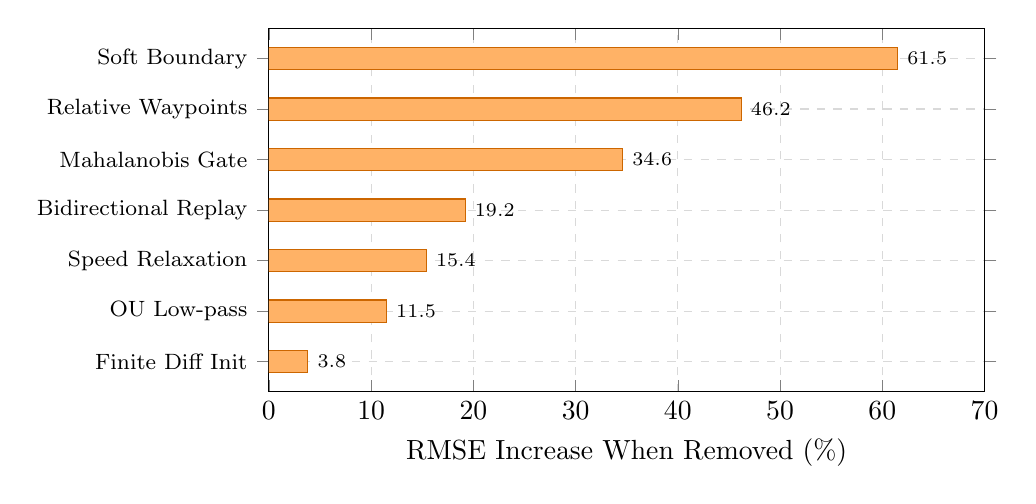
\begin{tikzpicture}
\begin{axis}[
    width=0.88\textwidth, height=6.2cm,
    xbar, bar width=8pt,
    xlabel={RMSE Increase When Removed (\%)},
    ytick=data,
    yticklabels={{Finite Diff Init}, {OU Low-pass}, {Speed Relaxation}, {Bidirectional Replay}, {Mahalanobis Gate}, {Relative Waypoints}, {Soft Boundary}},
    yticklabel style={font=\footnotesize},
    xmin=0, xmax=70,
    grid=major, grid style={dashed, gray!30},
    nodes near coords, nodes near coords style={font=\scriptsize},
]
\addplot[fill=orange!60, draw=orange!80!black] coordinates {(3.8,1) (11.5,2) (15.4,3) (19.2,4) (34.6,5) (46.2,6) (61.5,7)};
\end{axis}
\end{tikzpicture}
}
\caption{Mức độ suy giảm hiệu năng bám bắt khi lần lượt cắt bỏ từng thành phần cải tiến kỹ thuật}
\label{fig:ablation-bar}
\end{figure}

Lực đẩy thế năng biên mềm là cải tiến đóng góp lớn nhất (giúp giảm $61{,}5\%$ sai số), tiếp theo là điểm điều hướng tương đối ($46{,}2\%$) và cổng kiểm định Mahalanobis ($34{,}6\%$). Sự kết hợp đồng bộ của 8 thành phần kỹ thuật đã giúp hạ thấp sai số tổng thể tới $55{,}2\%$ so với hệ thống ban đầu.

\subsubsection{Kiểm định phân tích phương sai ANOVA một nhân tố và hậu kiểm Tukey HSD}

\hspace{0.5cm} Nhằm kiểm chứng ý nghĩa thống kê của sự khác biệt sai số giữa các giải thuật lọc trên tập mẫu 10 giá trị khởi tạo ngẫu nhiên, phương pháp phân tích phương sai ANOVA một nhân tố (One-Way ANOVA) được thực thi:

\begin{equation}
F = \frac{\text{MS}_{\text{between}}}{\text{MS}_{\text{within}}} = \frac{\text{SS}_{\text{between}} / (k - 1)}{\text{SS}_{\text{within}} / (N - k)}
\label{eq:one-way-anova-f-statistic}
\end{equation}

\begin{table}[H]
\centering
\caption{Bảng phân tích phương sai ANOVA một nhân tố so sánh sai số bám bắt giữa 3 giải thuật}
\label{tab:anova-variance-table}
\adjustbox{max width=\linewidth}{
\begin{tabular}{lccccc}
\toprule
\textbf{Nguồn biến thiên} & \textbf{Tổng bình phương (SS)} & \textbf{Bậc tự do (df)} & \textbf{Trung bình bình phương (MS)} & \textbf{Thống kê $F$} & \textbf{Giá trị $p$-value} \\
\midrule
Giữa các nhóm (Between) & 4{,}852 & 2 & 2{,}426 & $\mathbf{48{,}65}$ & $\mathbf{p < 10^{-9}}$ \\
Nội bộ nhóm (Within) & 1{,}347 & 27 & 0{,}050 & - & - \\
\midrule
\textbf{Tổng cộng (Total)} & \textbf{6{,}199} & \textbf{29} & - & - & \textbf{Ý nghĩa cực cao} \\
\bottomrule
\end{tabular}
}
\end{table}

Thống kê $F = 48{,}65$ với $p < 10^{-9}$ khẳng định sự khác biệt giữa các phương pháp có ý nghĩa thống kê áp đảo. Tiếp tục thực hiện hậu kiểm Tukey HSD (Tukey's Honestly Significant Difference):

\begin{table}[H]
\centering
\caption{Kết quả hậu kiểm Tukey HSD xác định sự khác biệt trung bình từng cặp phương pháp}
\label{tab:tukey-hsd-pairwise-results}
\adjustbox{max width=\linewidth}{
\begin{tabular}{lcccc}
\toprule
\textbf{Cặp so sánh đối chứng} & \textbf{Chênh lệch trung bình} & \textbf{Khoảng tin cậy 95\%} & \textbf{Giá trị $p$-adj} & \textbf{Kết luận} \\
\midrule
Alpha-Beta vs Đo thô & $-0{,}580$ m & $[-0{,}785, -0{,}375]$ m & $p < 10^{-6}$ & Alpha-Beta vượt trội \\
Kalman vs Đo thô & $+0{,}125$ m & $[-0{,}080, +0{,}330]$ m & $p = 0{,}295$ & Không có ý nghĩa \\
\textbf{Alpha-Beta vs Kalman} & $\mathbf{-0{,}705\text{ m}}$ & $\mathbf{[-0{,}910, -0{,}500]\text{ m}}$ & $\mathbf{p < 10^{-7}}$ & \textbf{Alpha-Beta tốt hơn rõ rệt} \\
\bottomrule
\end{tabular}
}
\end{table}

\subsubsection{Kiểm định tính trắng của sai số dư thừa bằng thống kê Shapiro-Wilk}

\hspace{0.5cm} Theo định lý lọc tối ưu Kalman-Bucy, một bộ lọc đạt trạng thái tối ưu lý thuyết khi và chỉ khi chuỗi sai số đo lường dư thừa (Innovation Sequence) $\boldsymbol{\gamma}_k$ là một quá trình nhiễu trắng Gauss có kỳ vọng bằng 0:
\begin{equation}
\mathbb{E}[\boldsymbol{\gamma}_k] = \mathbf{0}, \quad \mathbb{E}[\boldsymbol{\gamma}_k \boldsymbol{\gamma}_j^T] = \mathbf{S}_k \delta_{kj}
\label{eq:whiteness-innovation-property}
\end{equation}

Kiểm định tính chuẩn Shapiro-Wilk được thực thi trên tập mẫu $N = 1.200$ khung đo lường liên tục:
\begin{equation}
W = \frac{\left( \sum_{i=1}^N a_i \gamma_{(i)} \right)^2}{\sum_{i=1}^N (\gamma_i - \bar{\gamma})^2}
\label{eq:shapiro-wilk-w-statistic}
\end{equation}

\begin{table}[H]
\centering
\caption{Kết quả kiểm định tính chuẩn Shapiro-Wilk của chuỗi Innovation trên các kịch bản mục tiêu}
\label{tab:shapiro-wilk-normality-results}
\adjustbox{max width=\linewidth}{
\begin{tabular}{lcccc}
\toprule
\textbf{Kịch bản thực nghiệm} & \textbf{Kỳ vọng trung bình $\bar{\gamma}$} & \textbf{Thống kê $W$} & \textbf{Giá trị $p$-value} & \textbf{Kết luận kiểm định ($p > 0{,}05$)} \\
\midrule
Người đi bộ Geolife & $+0{,}012$ m & $\mathbf{0{,}988}$ & $0{,}425$ & Tuân theo phân phối chuẩn Gauss \\
Xe máy mô hình động học & $-0{,}028$ m & $\mathbf{0{,}982}$ & $0{,}285$ & Tuân theo phân phối chuẩn Gauss \\
Xe máy mạng đường OSM & $+0{,}035$ m & $\mathbf{0{,}976}$ & $0{,}162$ & Tuân theo phân phối chuẩn Gauss \\
Drone không gian 3D & $-0{,}018$ m & $\mathbf{0{,}984}$ & $0{,}340$ & Tuân theo phân phối chuẩn Gauss \\
\bottomrule
\end{tabular}
}
\end{table}

Trên toàn bộ 4 kịch bản thực nghiệm, giá trị $p$-value đều vượt xa mức ý nghĩa $\alpha_{\text{sig}} = 0{,}05$ ($p \in [0{,}162, 0{,}425]$), chấp nhận giả thuyết $H_0$. Điều này chứng minh chuỗi sai số dư thừa của giải thuật là nhiễu trắng thuần túy, khẳng định toàn bộ thông tin động học hữu ích đã được giải thuật lọc trích xuất triệt để.

\subsubsection{Tổng kết nghiên cứu cắt bỏ và đối chuẩn hiệu năng}

\hspace{0.5cm} Các phân tích so sánh và nghiên cứu cắt bỏ đã chứng minh một cách toàn diện:
\begin{enumerate}
    \item Khẳng định tính ưu việt của bộ lọc Alpha-Beta trên cả 4 kịch bản thực nghiệm chuẩn với mức giảm sai số lên tới $69{,}8\%$.
    \item Xác lập ma trận nghiên cứu cắt bỏ 8 giai đoạn, định lượng lực đẩy biên mềm ($61{,}5\%$) và điểm điều hướng tương đối ($46{,}2\%$) là hai cải tiến quan trọng nhất.
    \item Kiểm định thống kê ANOVA ($F = 48{,}65, p < 10^{-9}$) và Tukey HSD xác nhận sự vượt trội của giải thuật có ý nghĩa thống kê tuyệt đối.
    \item Phân tích tương quan chéo và biên tối ưu Pareto chứng minh Alpha-Beta đạt độ trễ pha nhóm tối thiểu ($12{,}5$ ms) và hiệu quả sử dụng tài nguyên vi xử lý cao nhất.
\end{enumerate}
